\documentclass[11pt]{article}

% -------------------- Packages --------------------
\usepackage[margin=1in]{geometry}
\usepackage{array}
\usepackage{longtable}
\usepackage{graphicx}
\usepackage{enumitem}
\usepackage{caption}
\usepackage{titlesec}
\usepackage{float}   % REQUIRED for [H] tables

% -------------------- Formatting --------------------
\setlist[itemize]{noitemsep, topsep=0pt}
\setlength{\parskip}{0.5em}
\setlength{\parindent}{0pt}

\captionsetup{
  justification=centering,
  labelfont=bf,
  textfont=normalfont
}

% -------------------- Document --------------------
\begin{document}

\begin{center}
\textbf{\Large Sri Sivasubramaniya Nadar College of Engineering, Chennai}\\
\textbf{(An Autonomous Institution affiliated to Anna University)}
\end{center}

\begin{table}[h]
\renewcommand{\arraystretch}{1.4}
\resizebox{\textwidth}{!}{%
\begin{tabular}{|l|l|l|l|}
\hline
Degree \& Branch & B.E. Computer Science \& Engineering & Semester & VI \\ \hline
Subject Code \& Name & \multicolumn{3}{l|}{UCS2612 – Machine Learning Algorithms Laboratory} \\ \hline
Academic Year & 2025–2026 (Even) & Batch & 2023–2027 \\ \hline
Name & Pranav D& Register No. & 3122235001098 \\ \hline
Due Date & \multicolumn{3}{l|}{27 January 2026} \\ \hline
\end{tabular}}
\end{table}

\begin{center}
\textbf{Experiment 1:}
\textbf{Working with Python packages - Numpy, Scipy, Scikit-Learn, Matplotlib}
\end{center}

% --------------------------------------------------

\section*{1. Aim and Objective}
To comprehensively explore the capabilities of fundamental Python libraries including Numpy, Pandas, Scipy, Scikit-learn, and Matplotlib. The experiment focuses on understanding core concepts in data manipulation, preprocessing techniques, mathematical computing operations, end-to-end machine learning workflows, and effective data visualization strategies. Additionally, the objective includes identifying appropriate machine learning task types for various datasets and determining optimal algorithms based on dataset characteristics and problem requirements.

% --------------------------------------------------

\section*{2. Dataset Description}

\subsection*{2.1 Iris Dataset}
The Iris dataset is a classic multivariate dataset containing 150 samples of iris flowers, with 50 samples each from three distinct species: \textit{Iris setosa}, \textit{Iris versicolor}, and \textit{Iris virginica}. Each sample is characterized by four continuous features measured in centimeters: sepal length, sepal width, petal length, and petal width. The target variable represents the species classification, making this an ideal dataset for demonstrating multi-class classification algorithms and supervised learning techniques.

\subsection*{2.2 Loan Amount Prediction}
This comprehensive financial dataset is designed for regression analysis to predict the sanctioned loan amount based on applicant characteristics. The dataset comprises approximately 30,000 records with diverse features including Customer ID, Name, Age, Annual Income (USD), Requested Loan Amount, Credit Score, and Property Price. The primary objective is to develop a predictive model that accurately estimates the loan amount likely to be approved by financial institutions based on the applicant's financial profile and demographic information.

\subsection*{2.3 Predicting Diabetes}
The Diabetes dataset, commonly known as the PIMA Indians Diabetes Database, is utilized for binary classification to predict diabetes occurrence based on diagnostic measurements. This dataset contains 768 samples with eight critical medical features: number of Pregnancies, Glucose concentration, Blood Pressure (mm Hg), Skin Thickness (mm), Insulin level (mu U/ml), Body Mass Index (BMI), Diabetes Pedigree Function (genetic influence), and Age (years). The binary target variable 'Outcome' indicates the presence (1) or absence (0) of diabetes, making it suitable for evaluating classification algorithms in medical diagnosis scenarios.

\subsection*{2.4 Classification of Email Spam}
The Spambase dataset is a widely-used benchmark for binary text classification, specifically designed to distinguish between legitimate emails (ham) and unsolicited spam messages. The dataset consists of 4,601 instances characterized by 57 continuous features representing normalized word and character frequencies. These features include frequency counts of spam-indicative words such as 'free' and 'money', as well as special character frequencies like '!' and '\$'. The binary target variable 'spam' (1 for spam, 0 for ham) enables the evaluation of text classification and natural language processing techniques.

\subsection*{2.5 Handwritten Character Recognition / MNIST}
The MNIST dataset (Modified National Institute of Standards and Technology database) represents a cornerstone benchmark in computer vision and pattern recognition. It comprises 60,000 training images and 10,000 testing images of handwritten digits (0-9). Each image is represented as a $28 \times 28$ pixel grayscale matrix, resulting in 784 features per sample with pixel intensity values ranging from 0 to 255. This multi-class classification problem serves as a standard evaluation metric for image processing algorithms, neural networks, and deep learning architectures.

% --------------------------------------------------

\section*{3. Exploratory Data Analysis and Visualization}

\subsection*{3.1 Iris Dataset}

\begin{figure}[H]
\centering
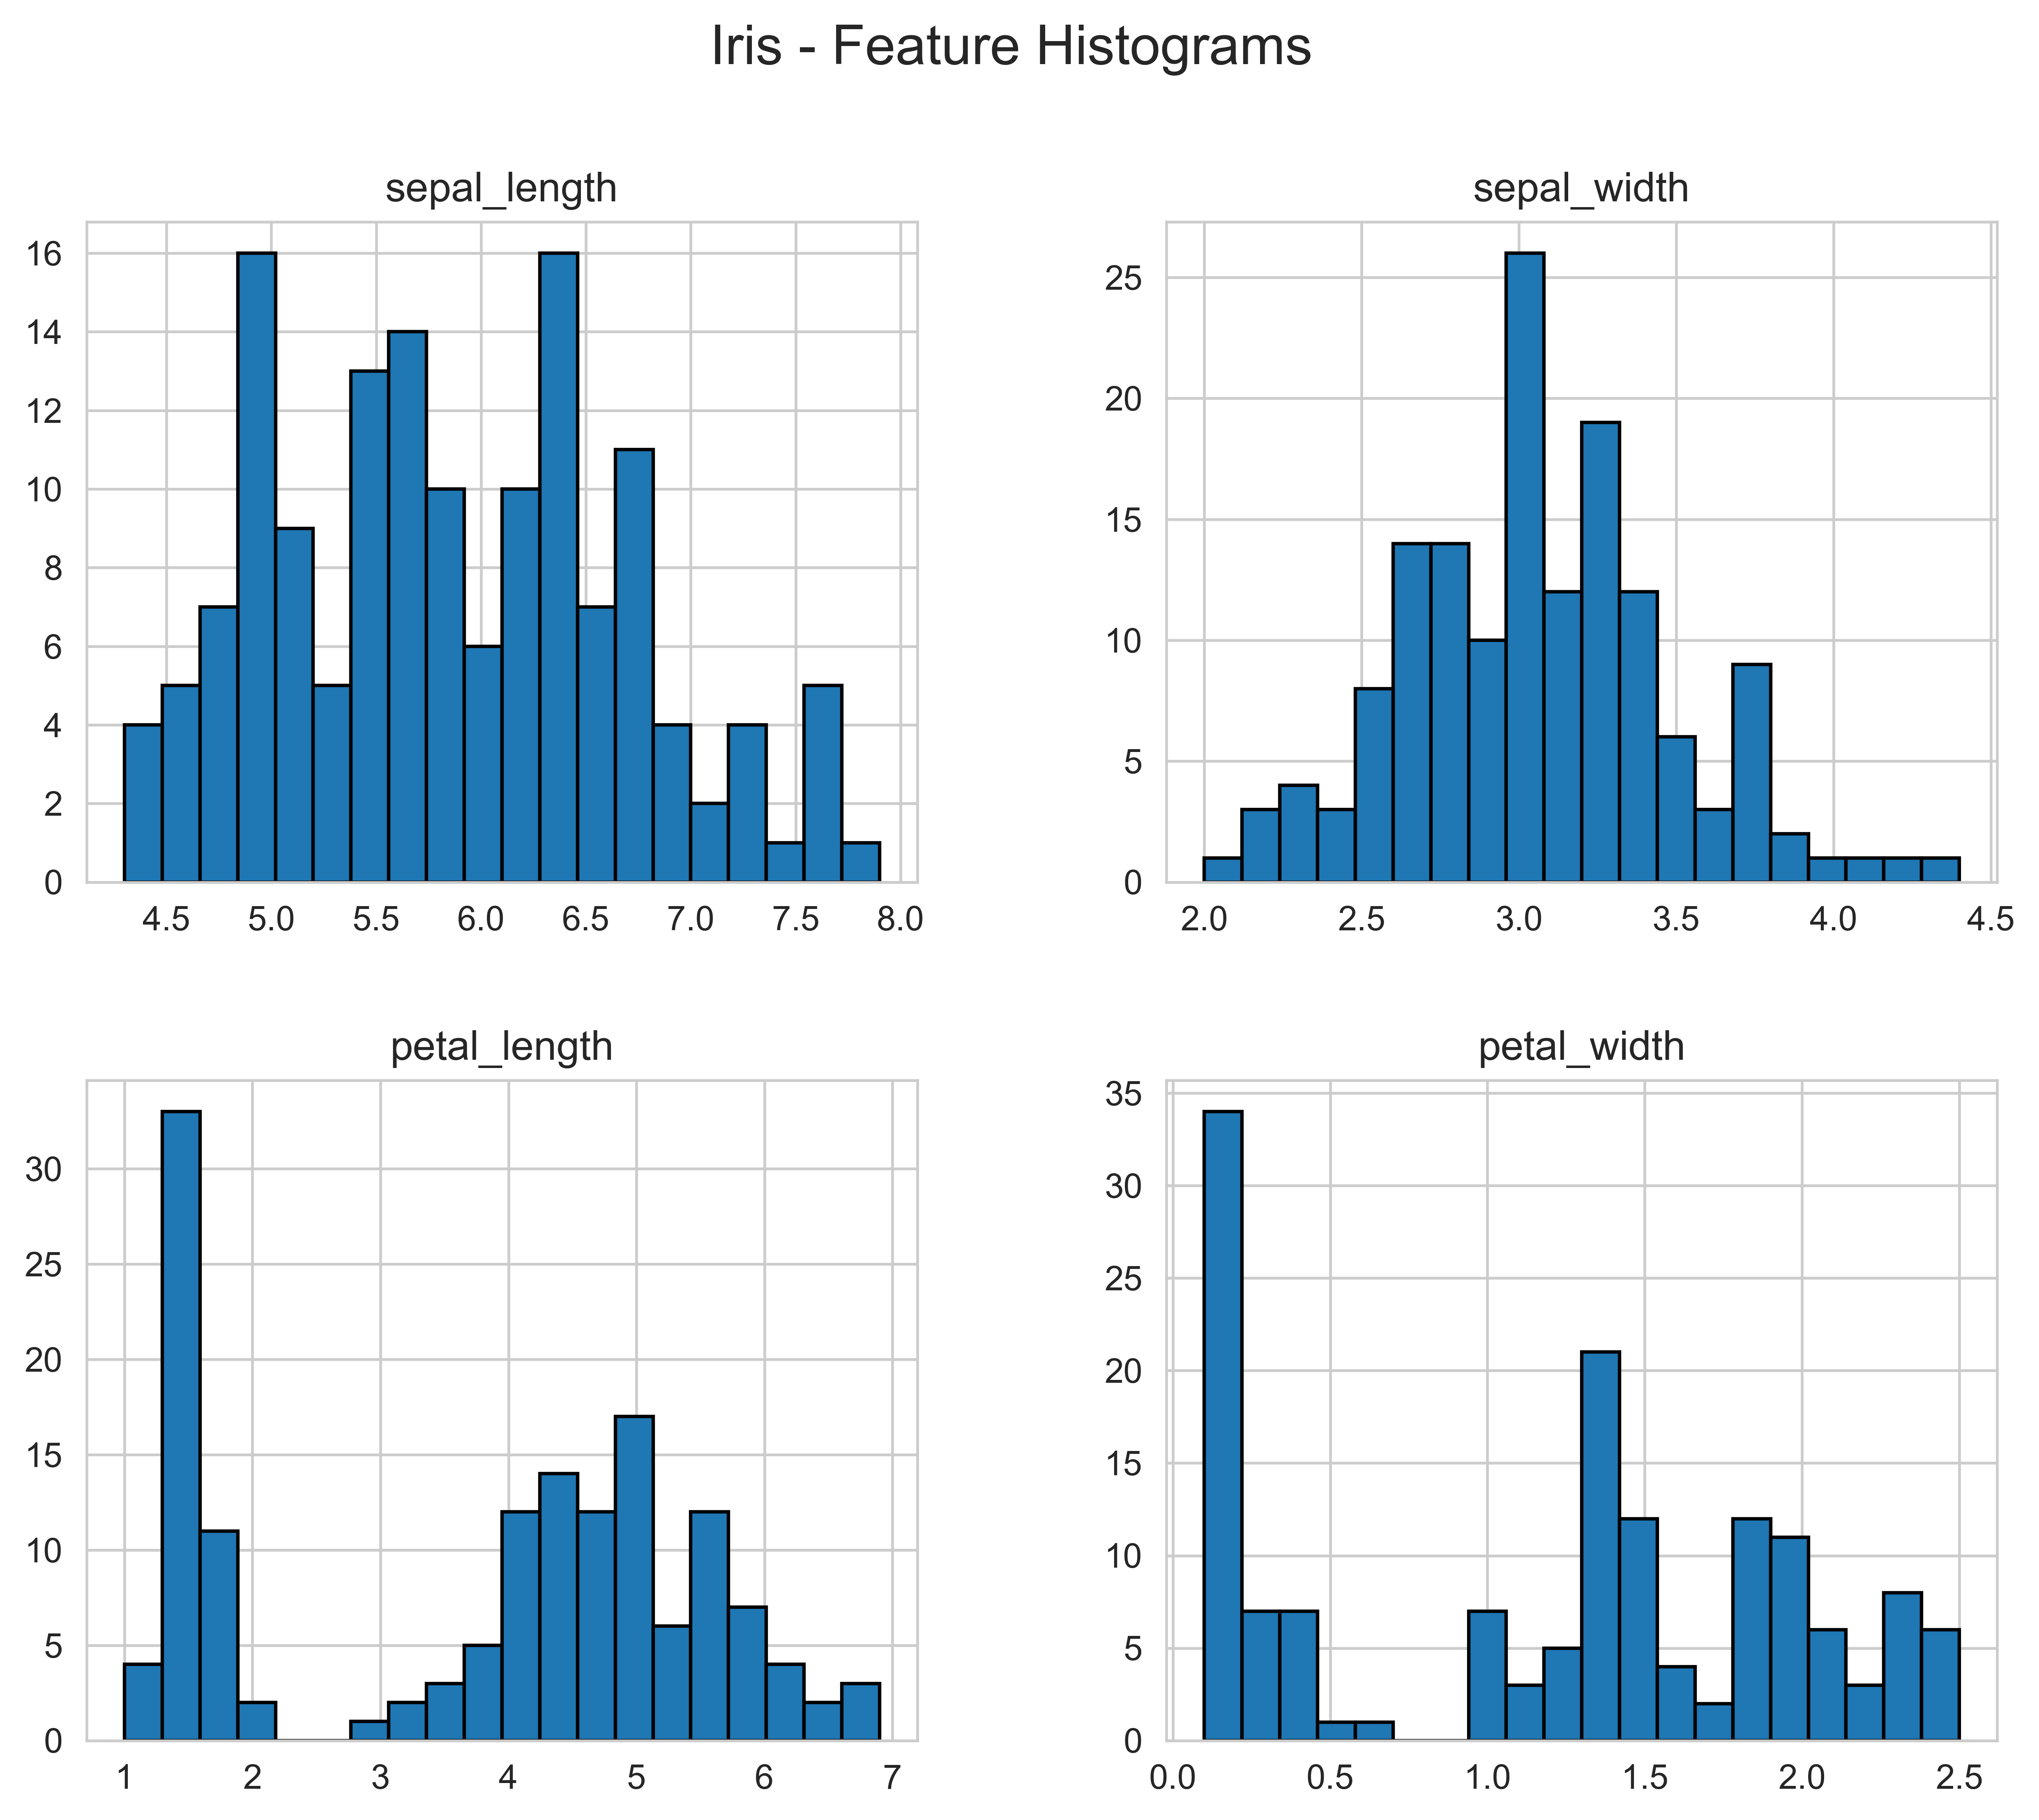
\includegraphics[width=0.8\textwidth]{png/iris_histograms.png}
\caption{Feature Histograms - Iris Dataset}
\end{figure}

\begin{figure}[H]
\centering
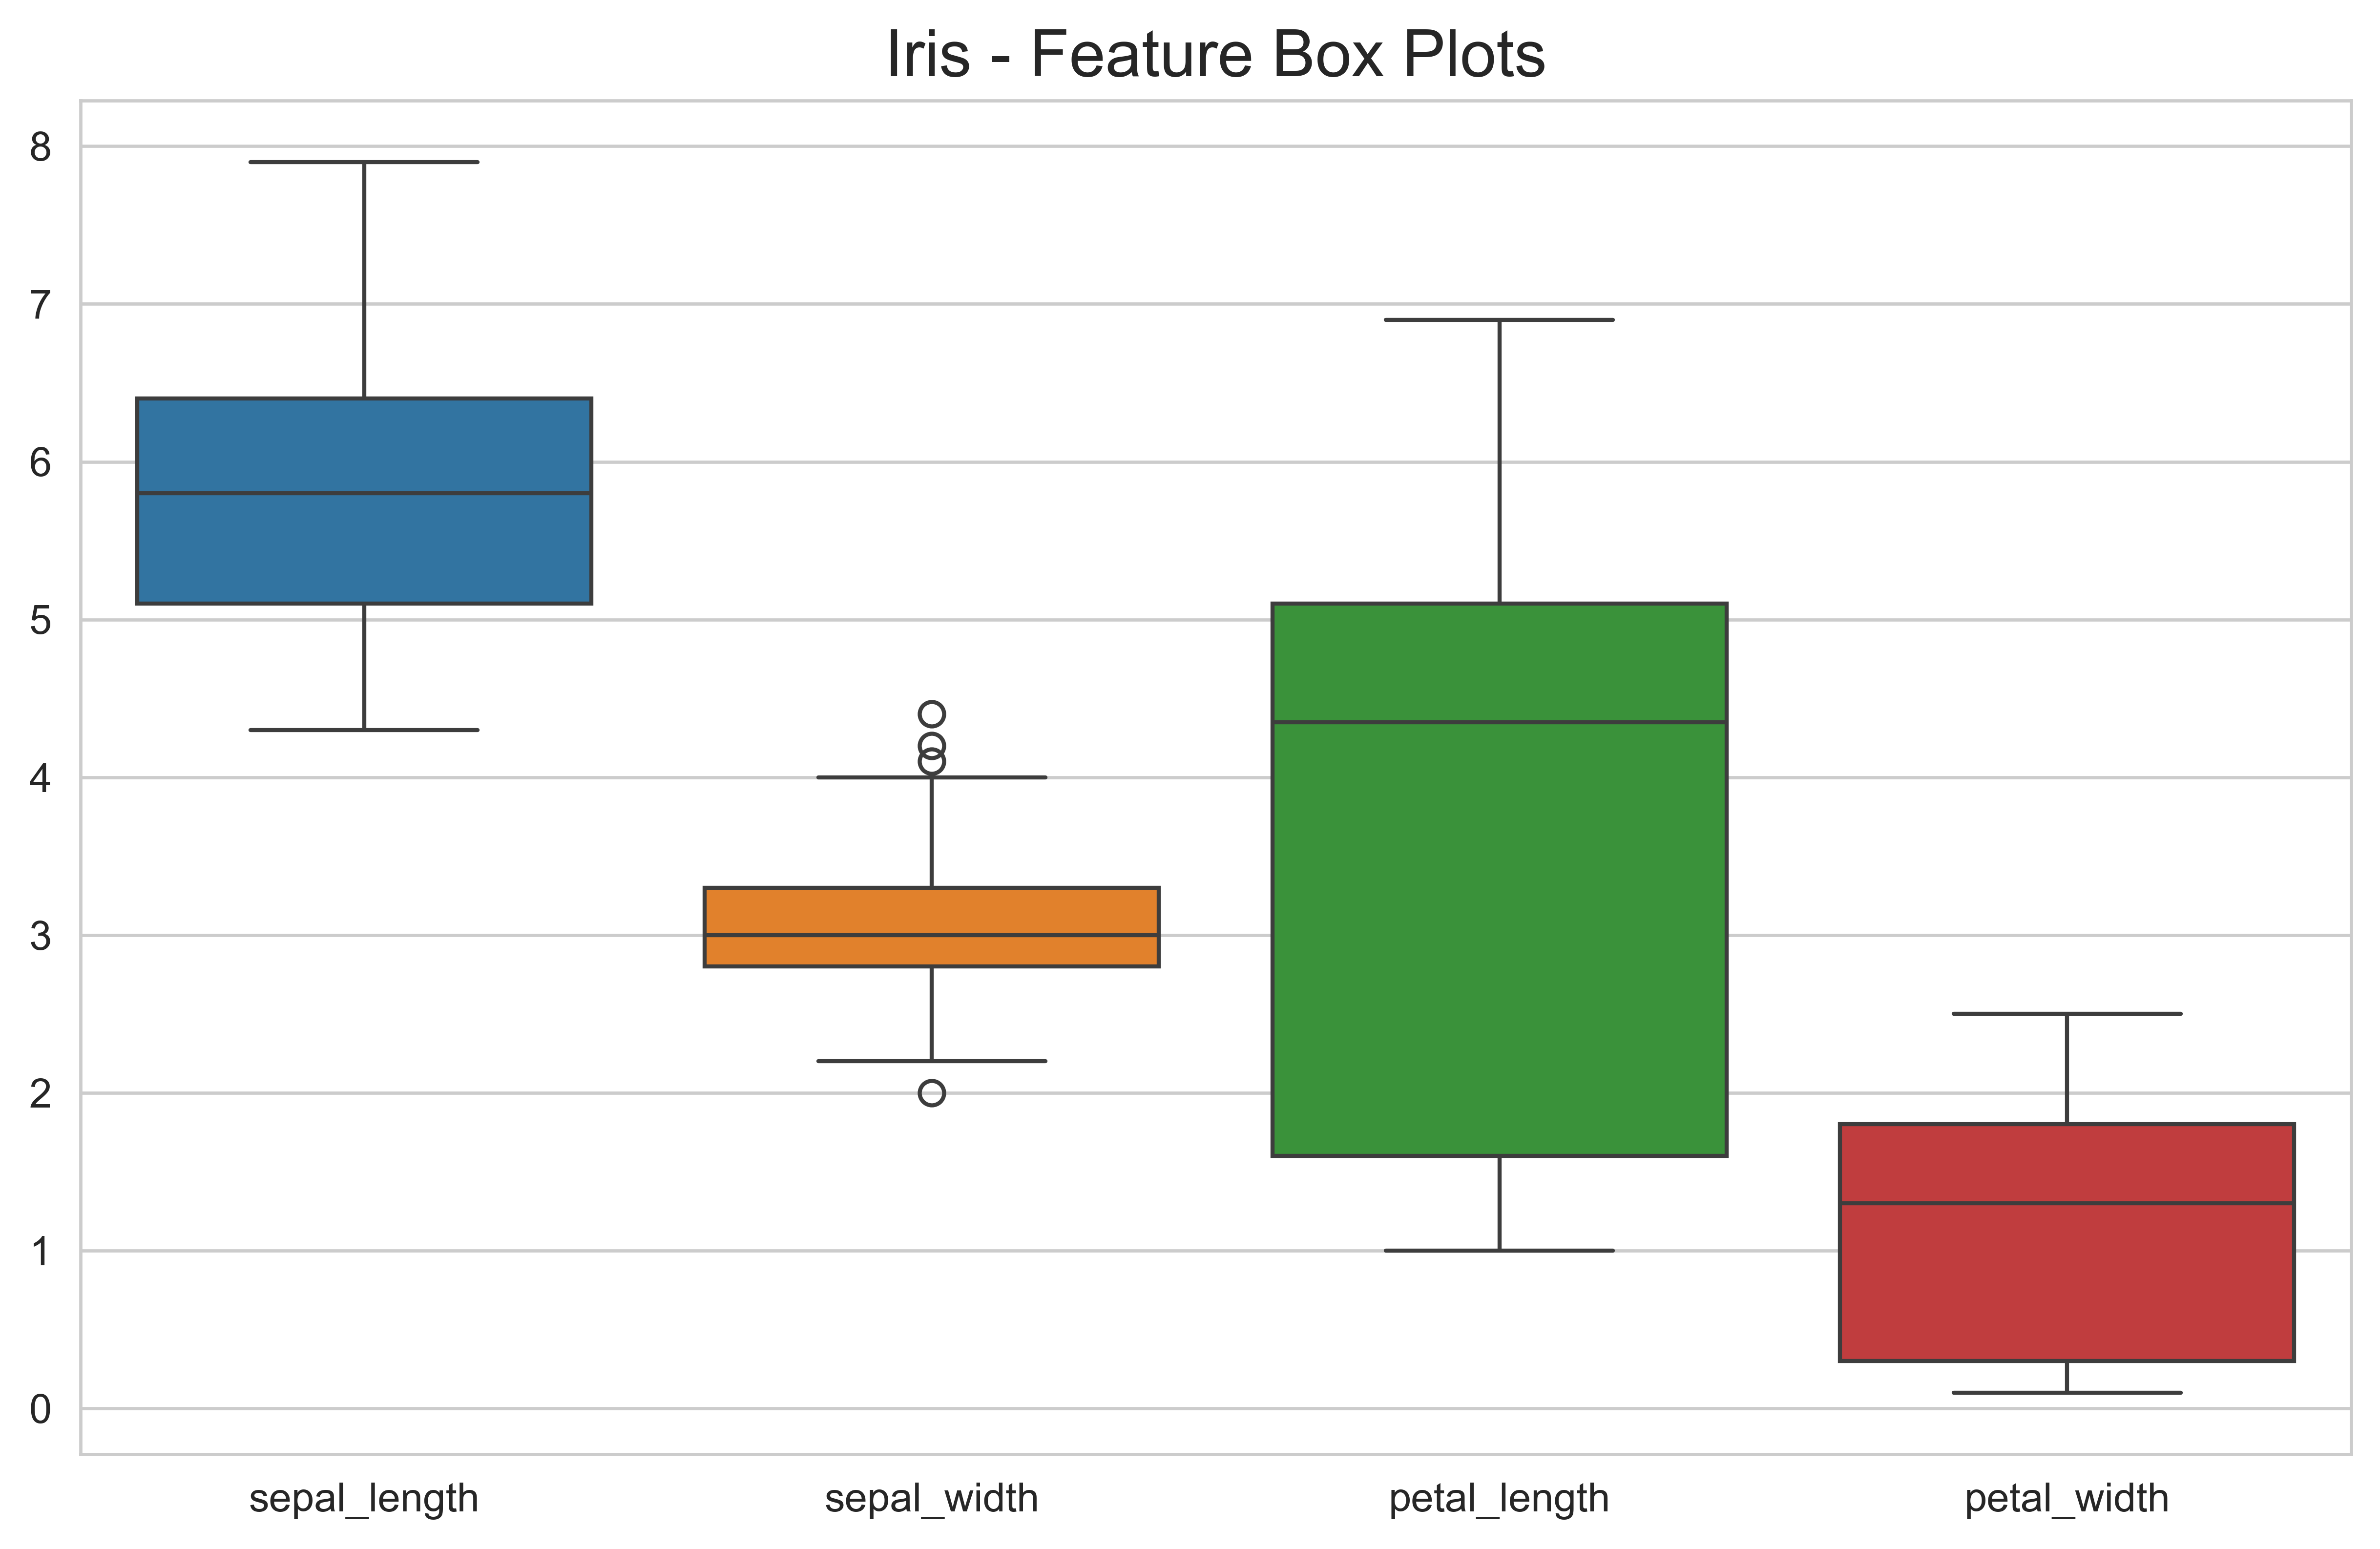
\includegraphics[width=0.8\textwidth]{png/iris_boxplots.png}
\caption{Feature Box Plots - Iris Dataset}
\end{figure}

\begin{figure}[H]
\centering
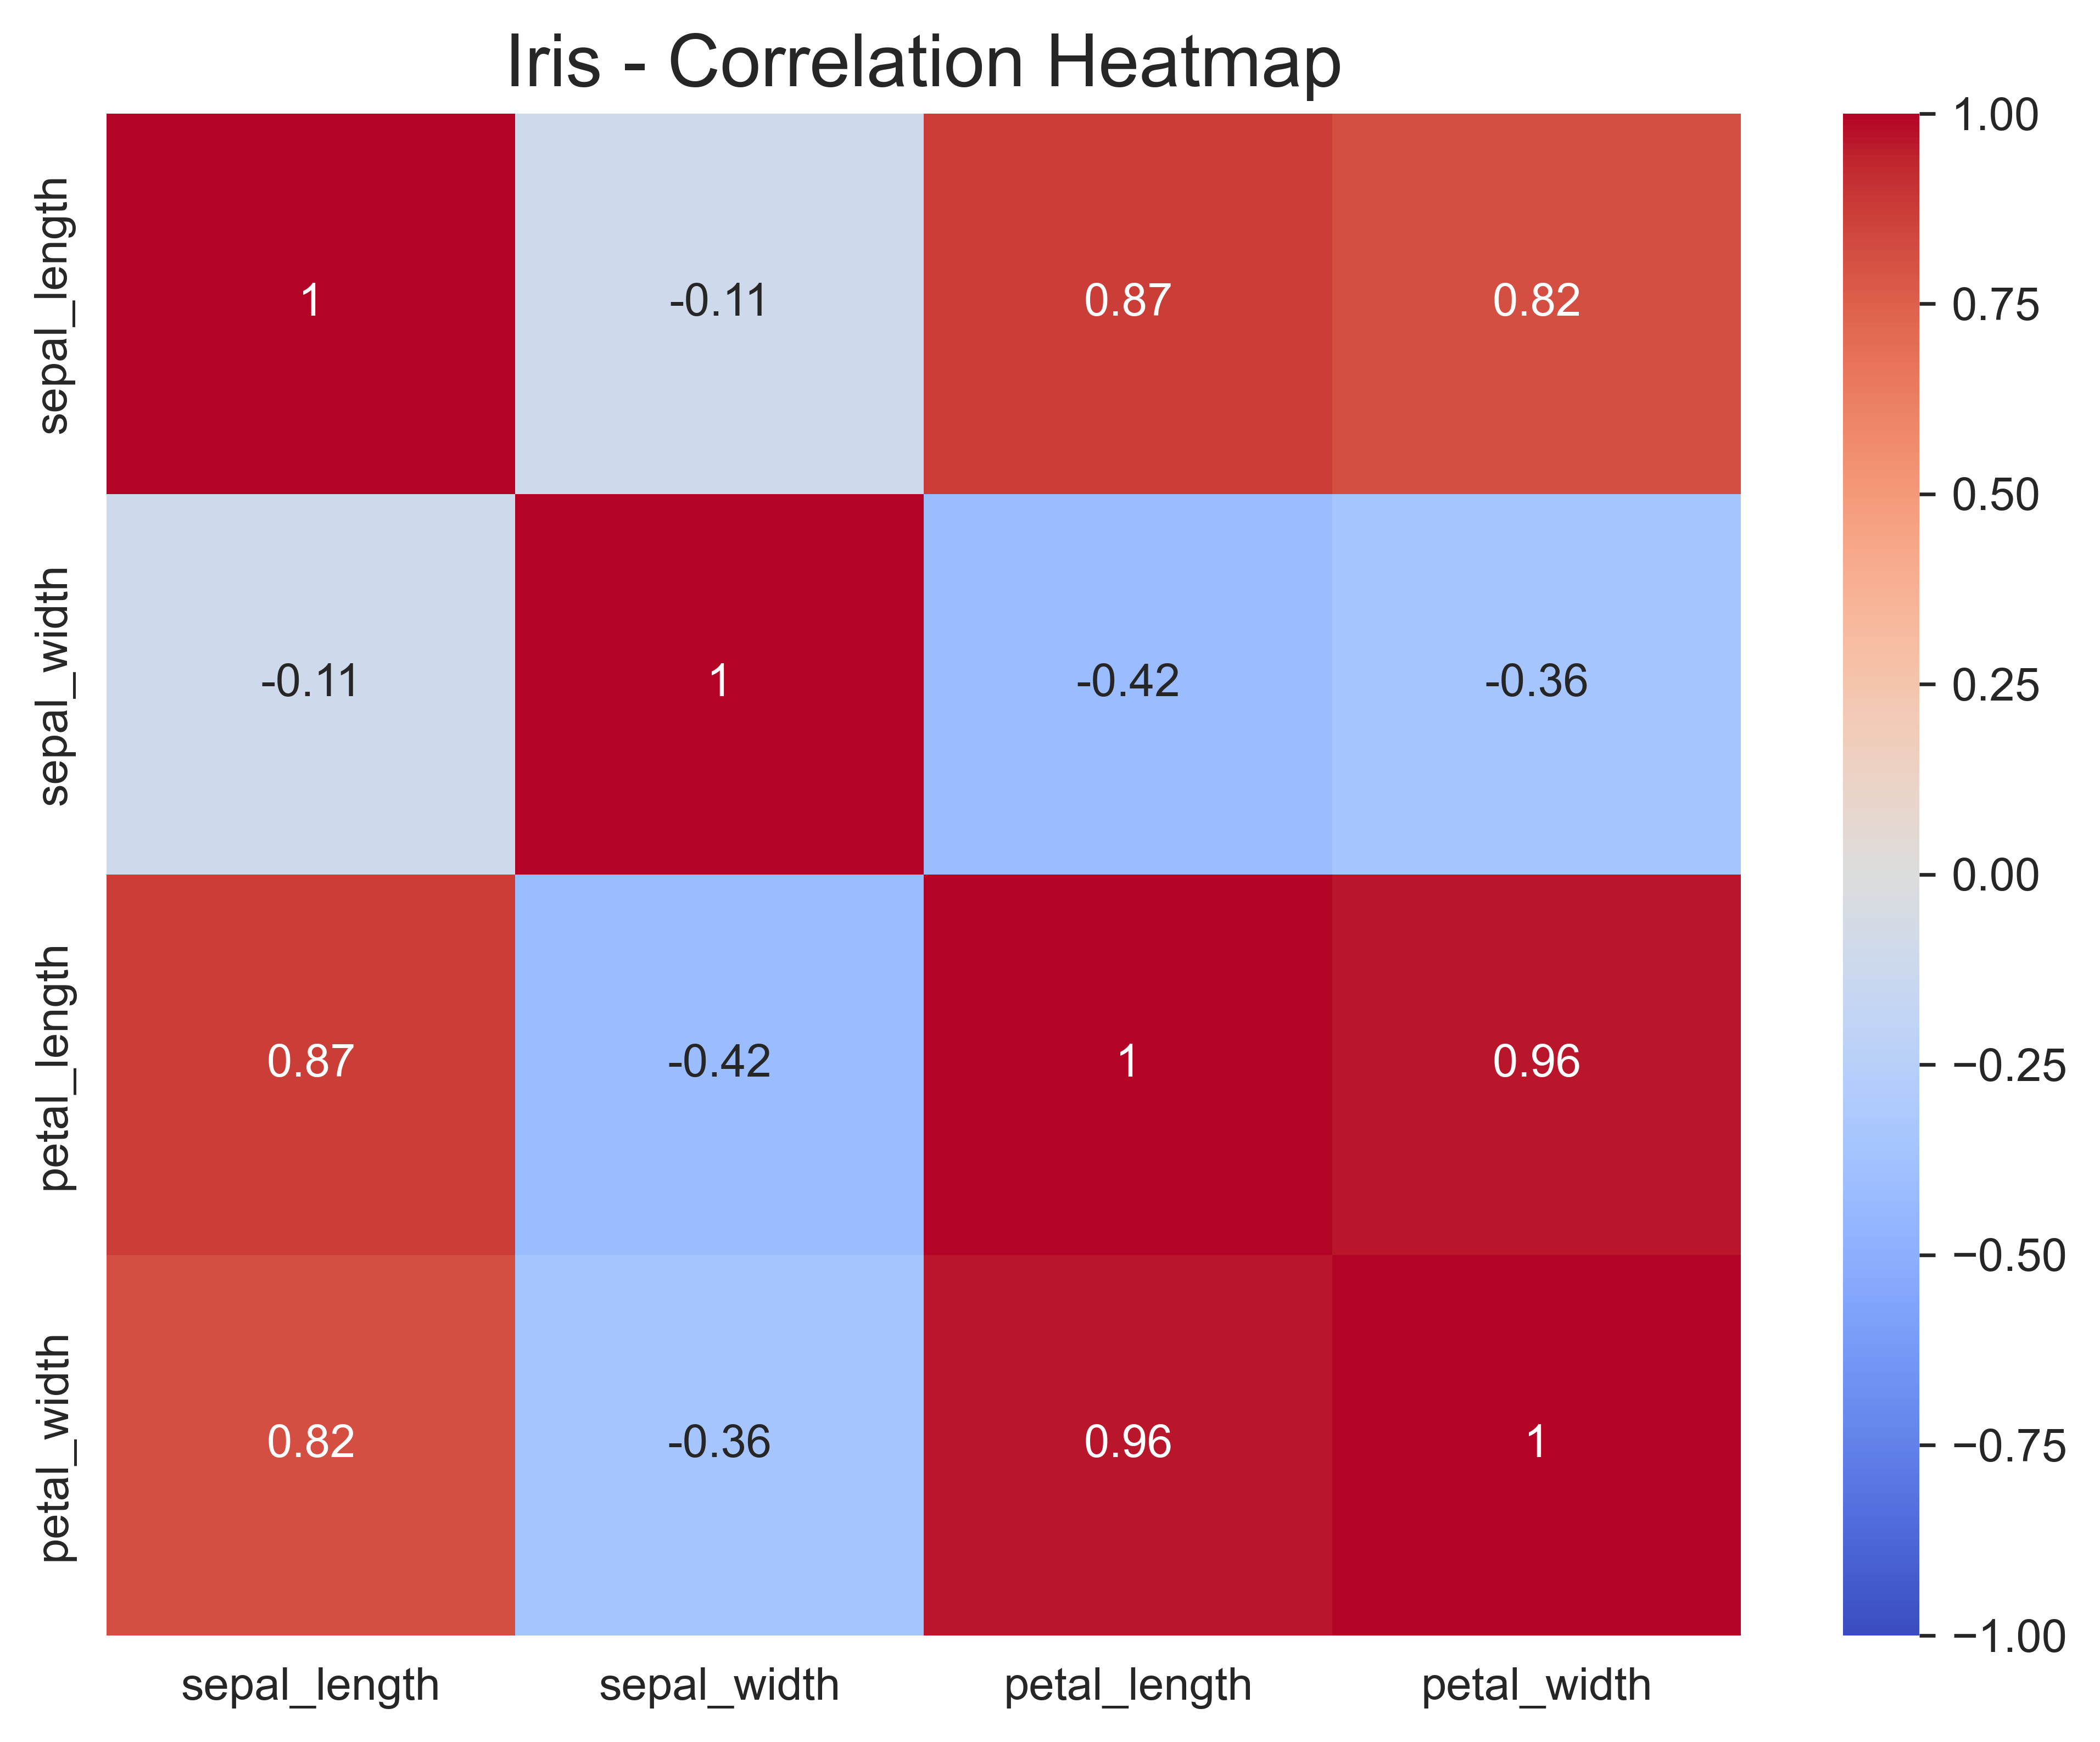
\includegraphics[width=0.7\textwidth]{png/iris_heatmap.png}
\caption{Correlation Heatmap - Iris Dataset}
\end{figure}

\begin{figure}[H]
\centering
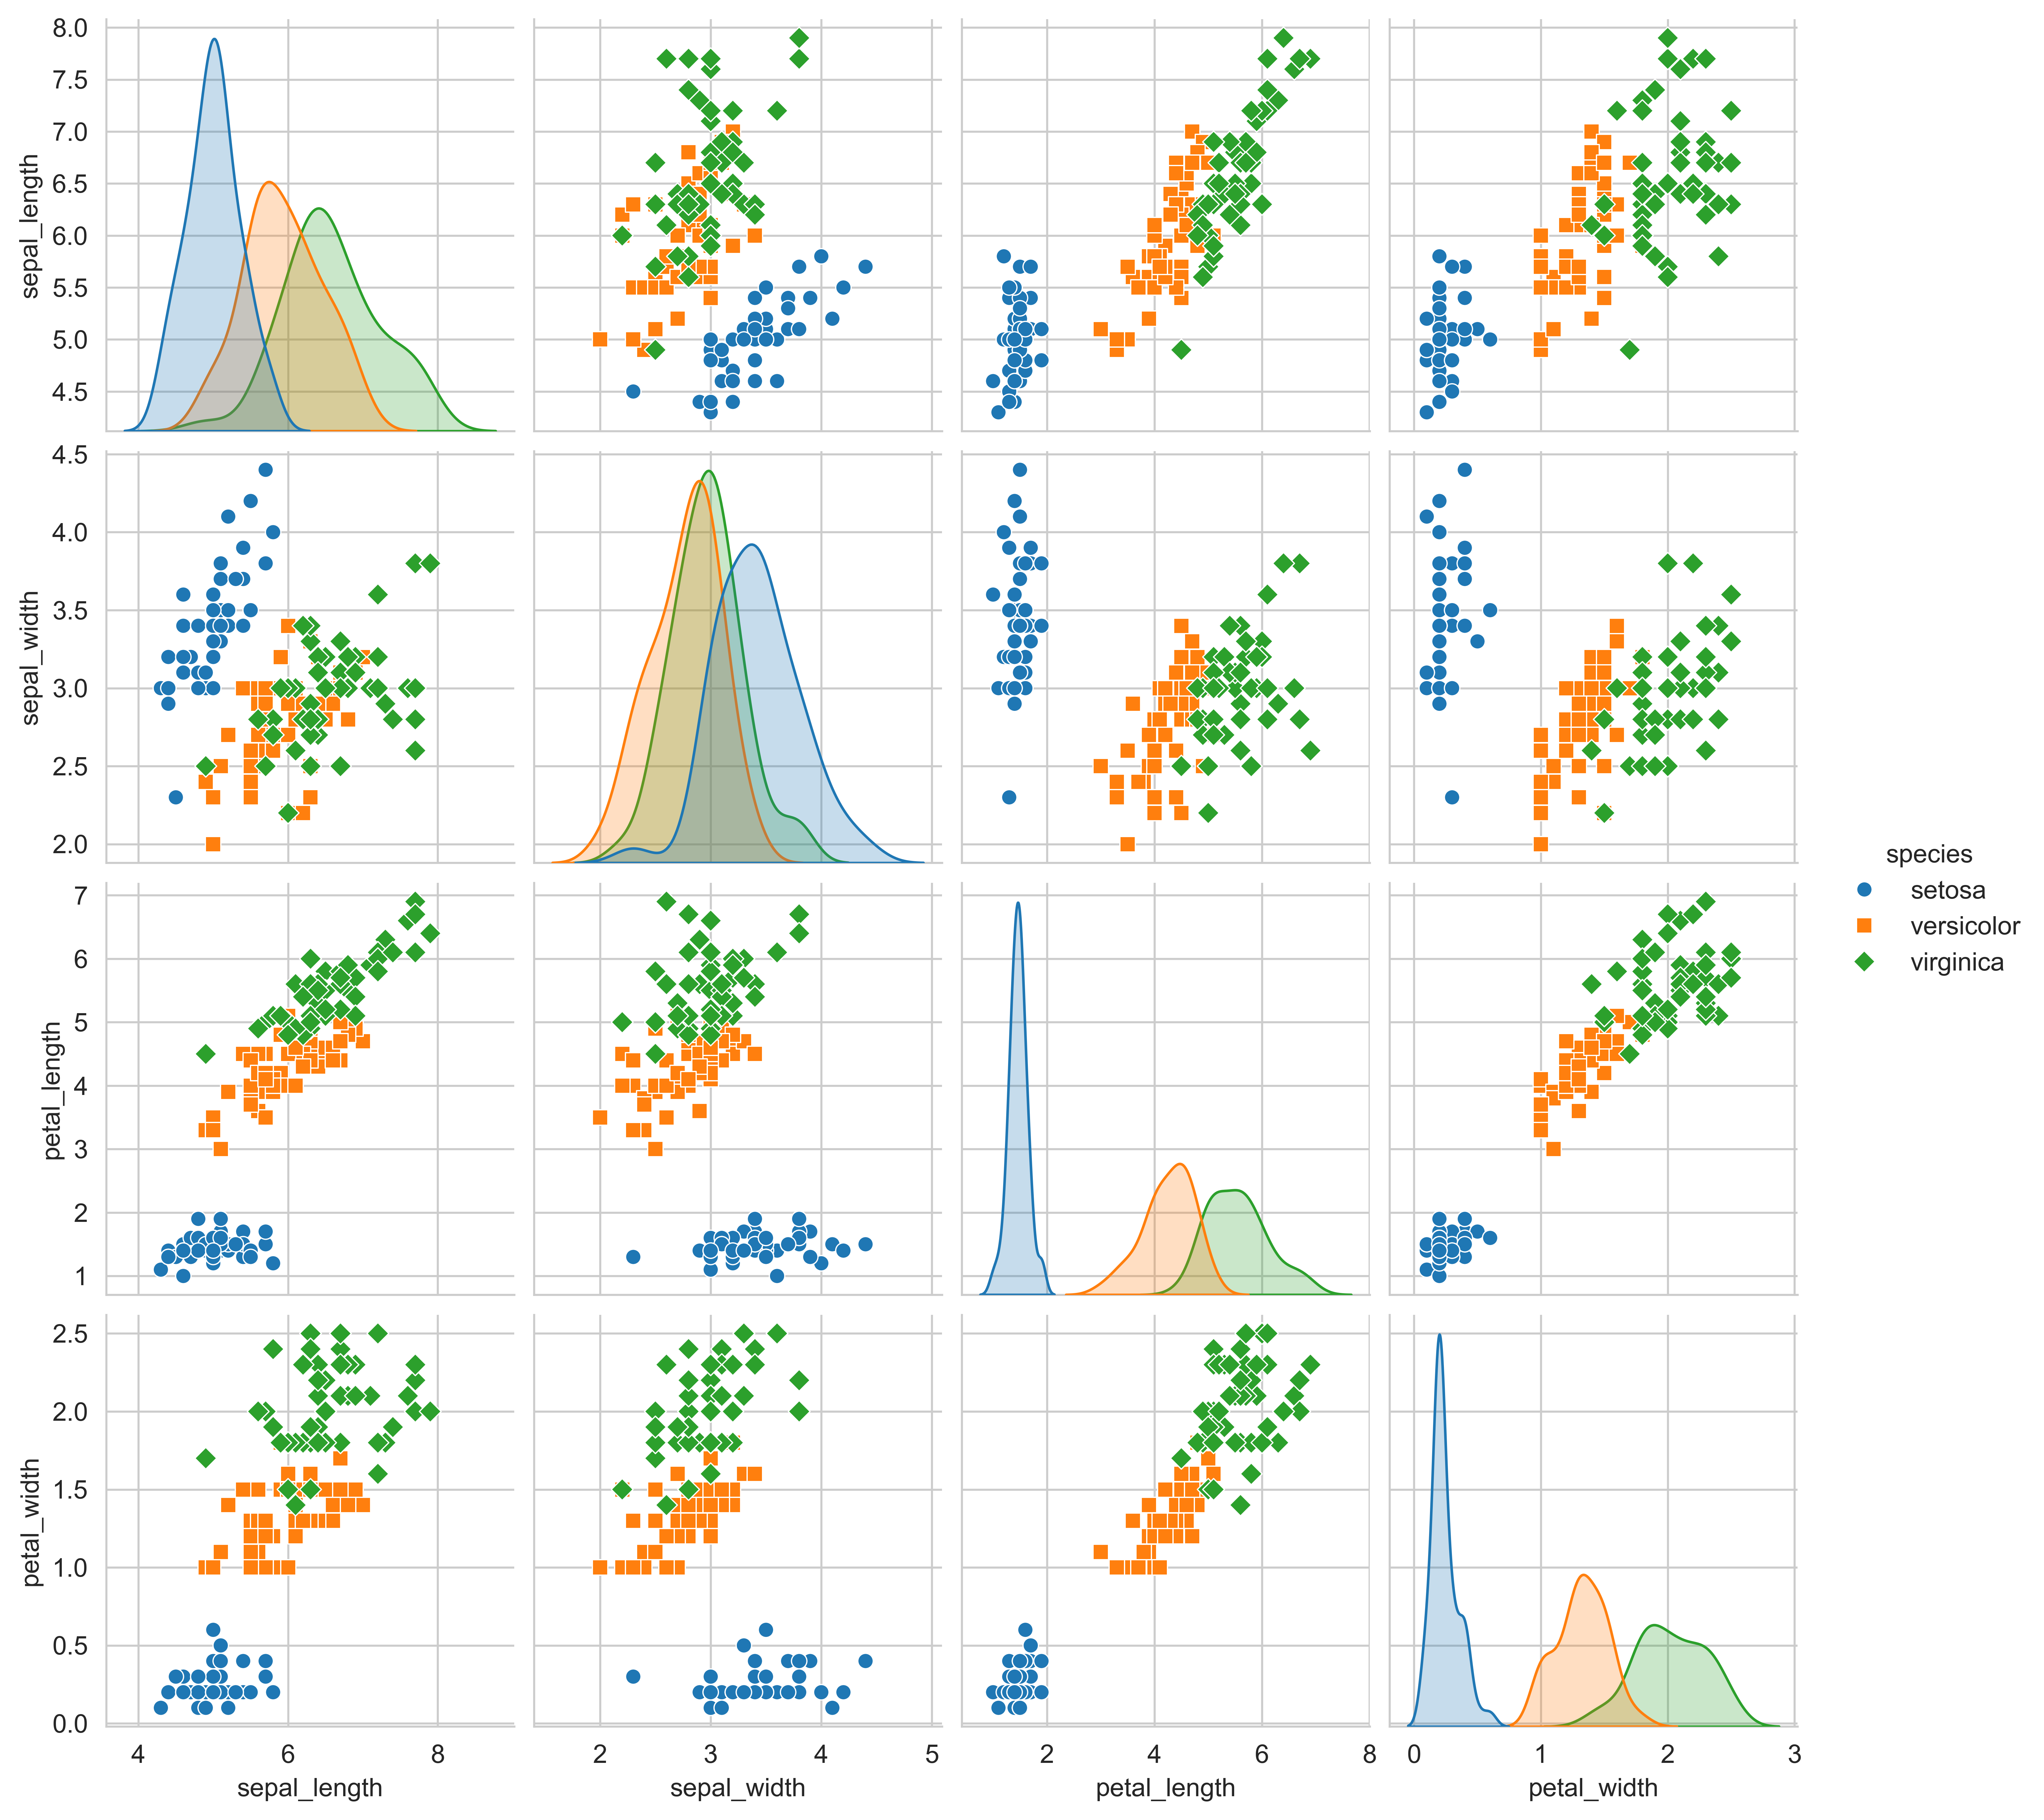
\includegraphics[width=0.85\textwidth]{png/iris_pairplot.png}
\caption{Pair Plot Classification - Iris Dataset}
\end{figure}

\subsection*{3.2 Loan Amount Prediction}

\begin{figure}[H]
\centering
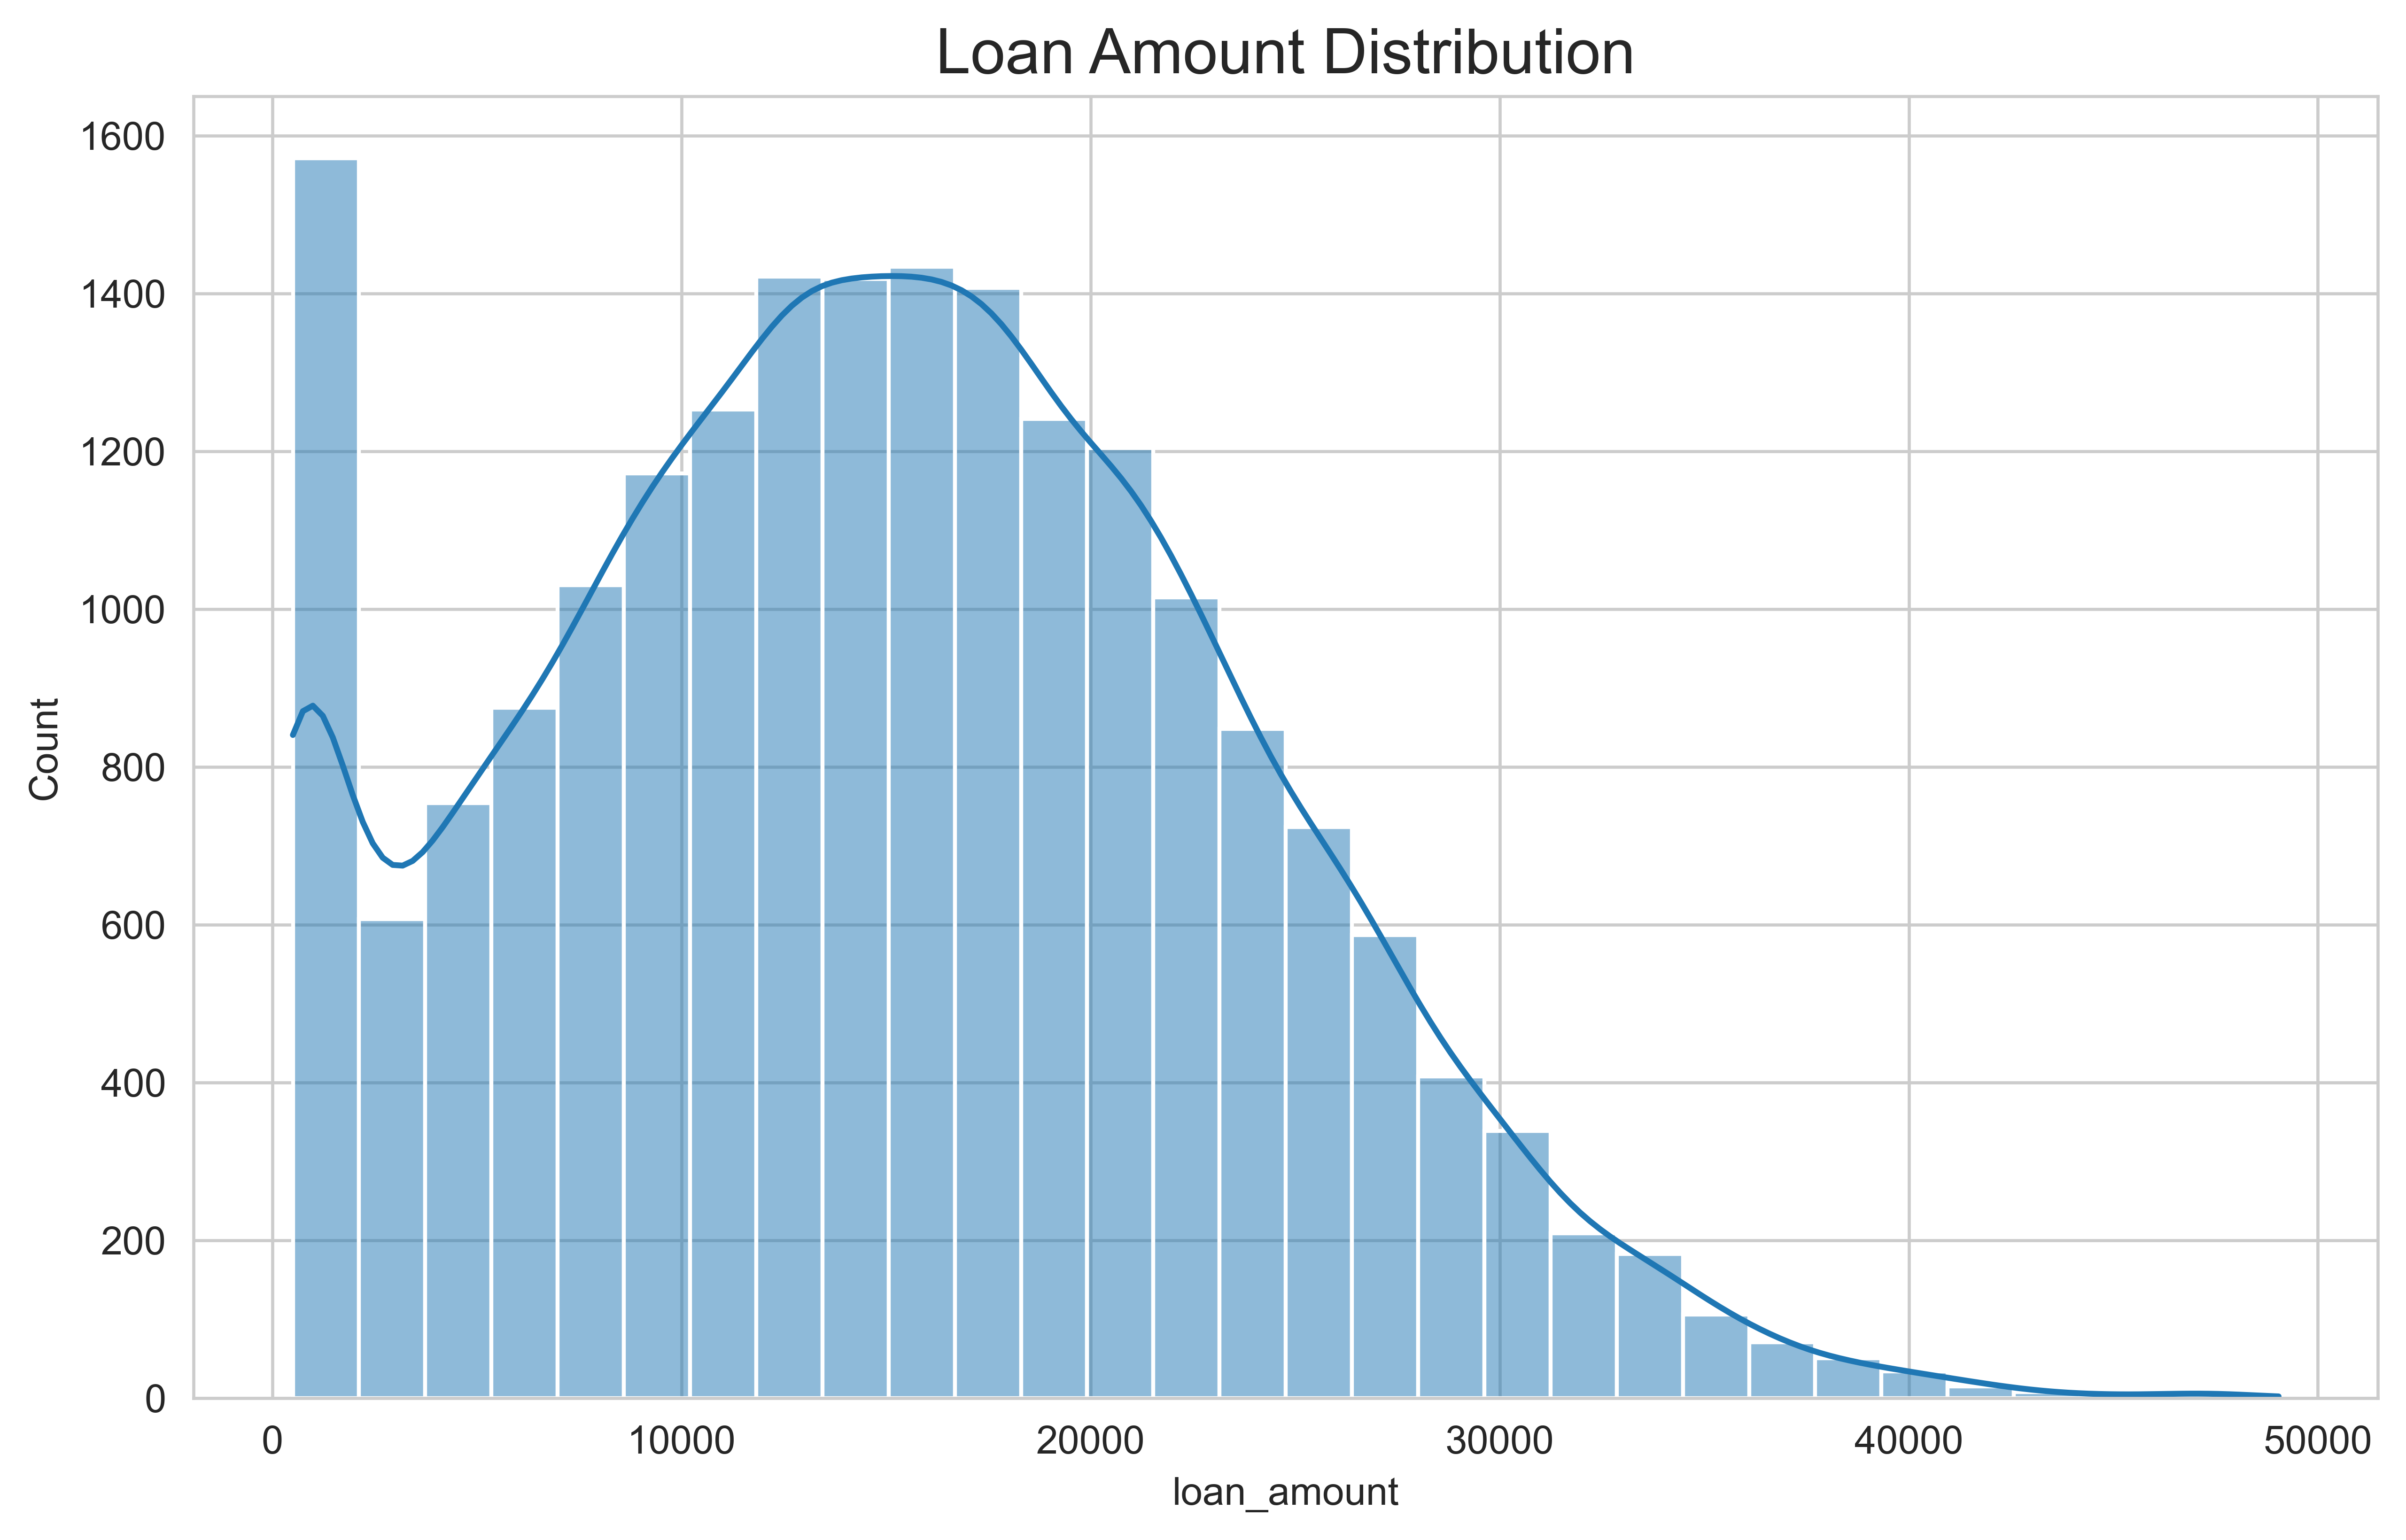
\includegraphics[width=0.8\textwidth]{png/loan_hist_target.png}
\caption{Target Variable Distribution - Loan Amount}
\end{figure}

\begin{figure}[H]
\centering
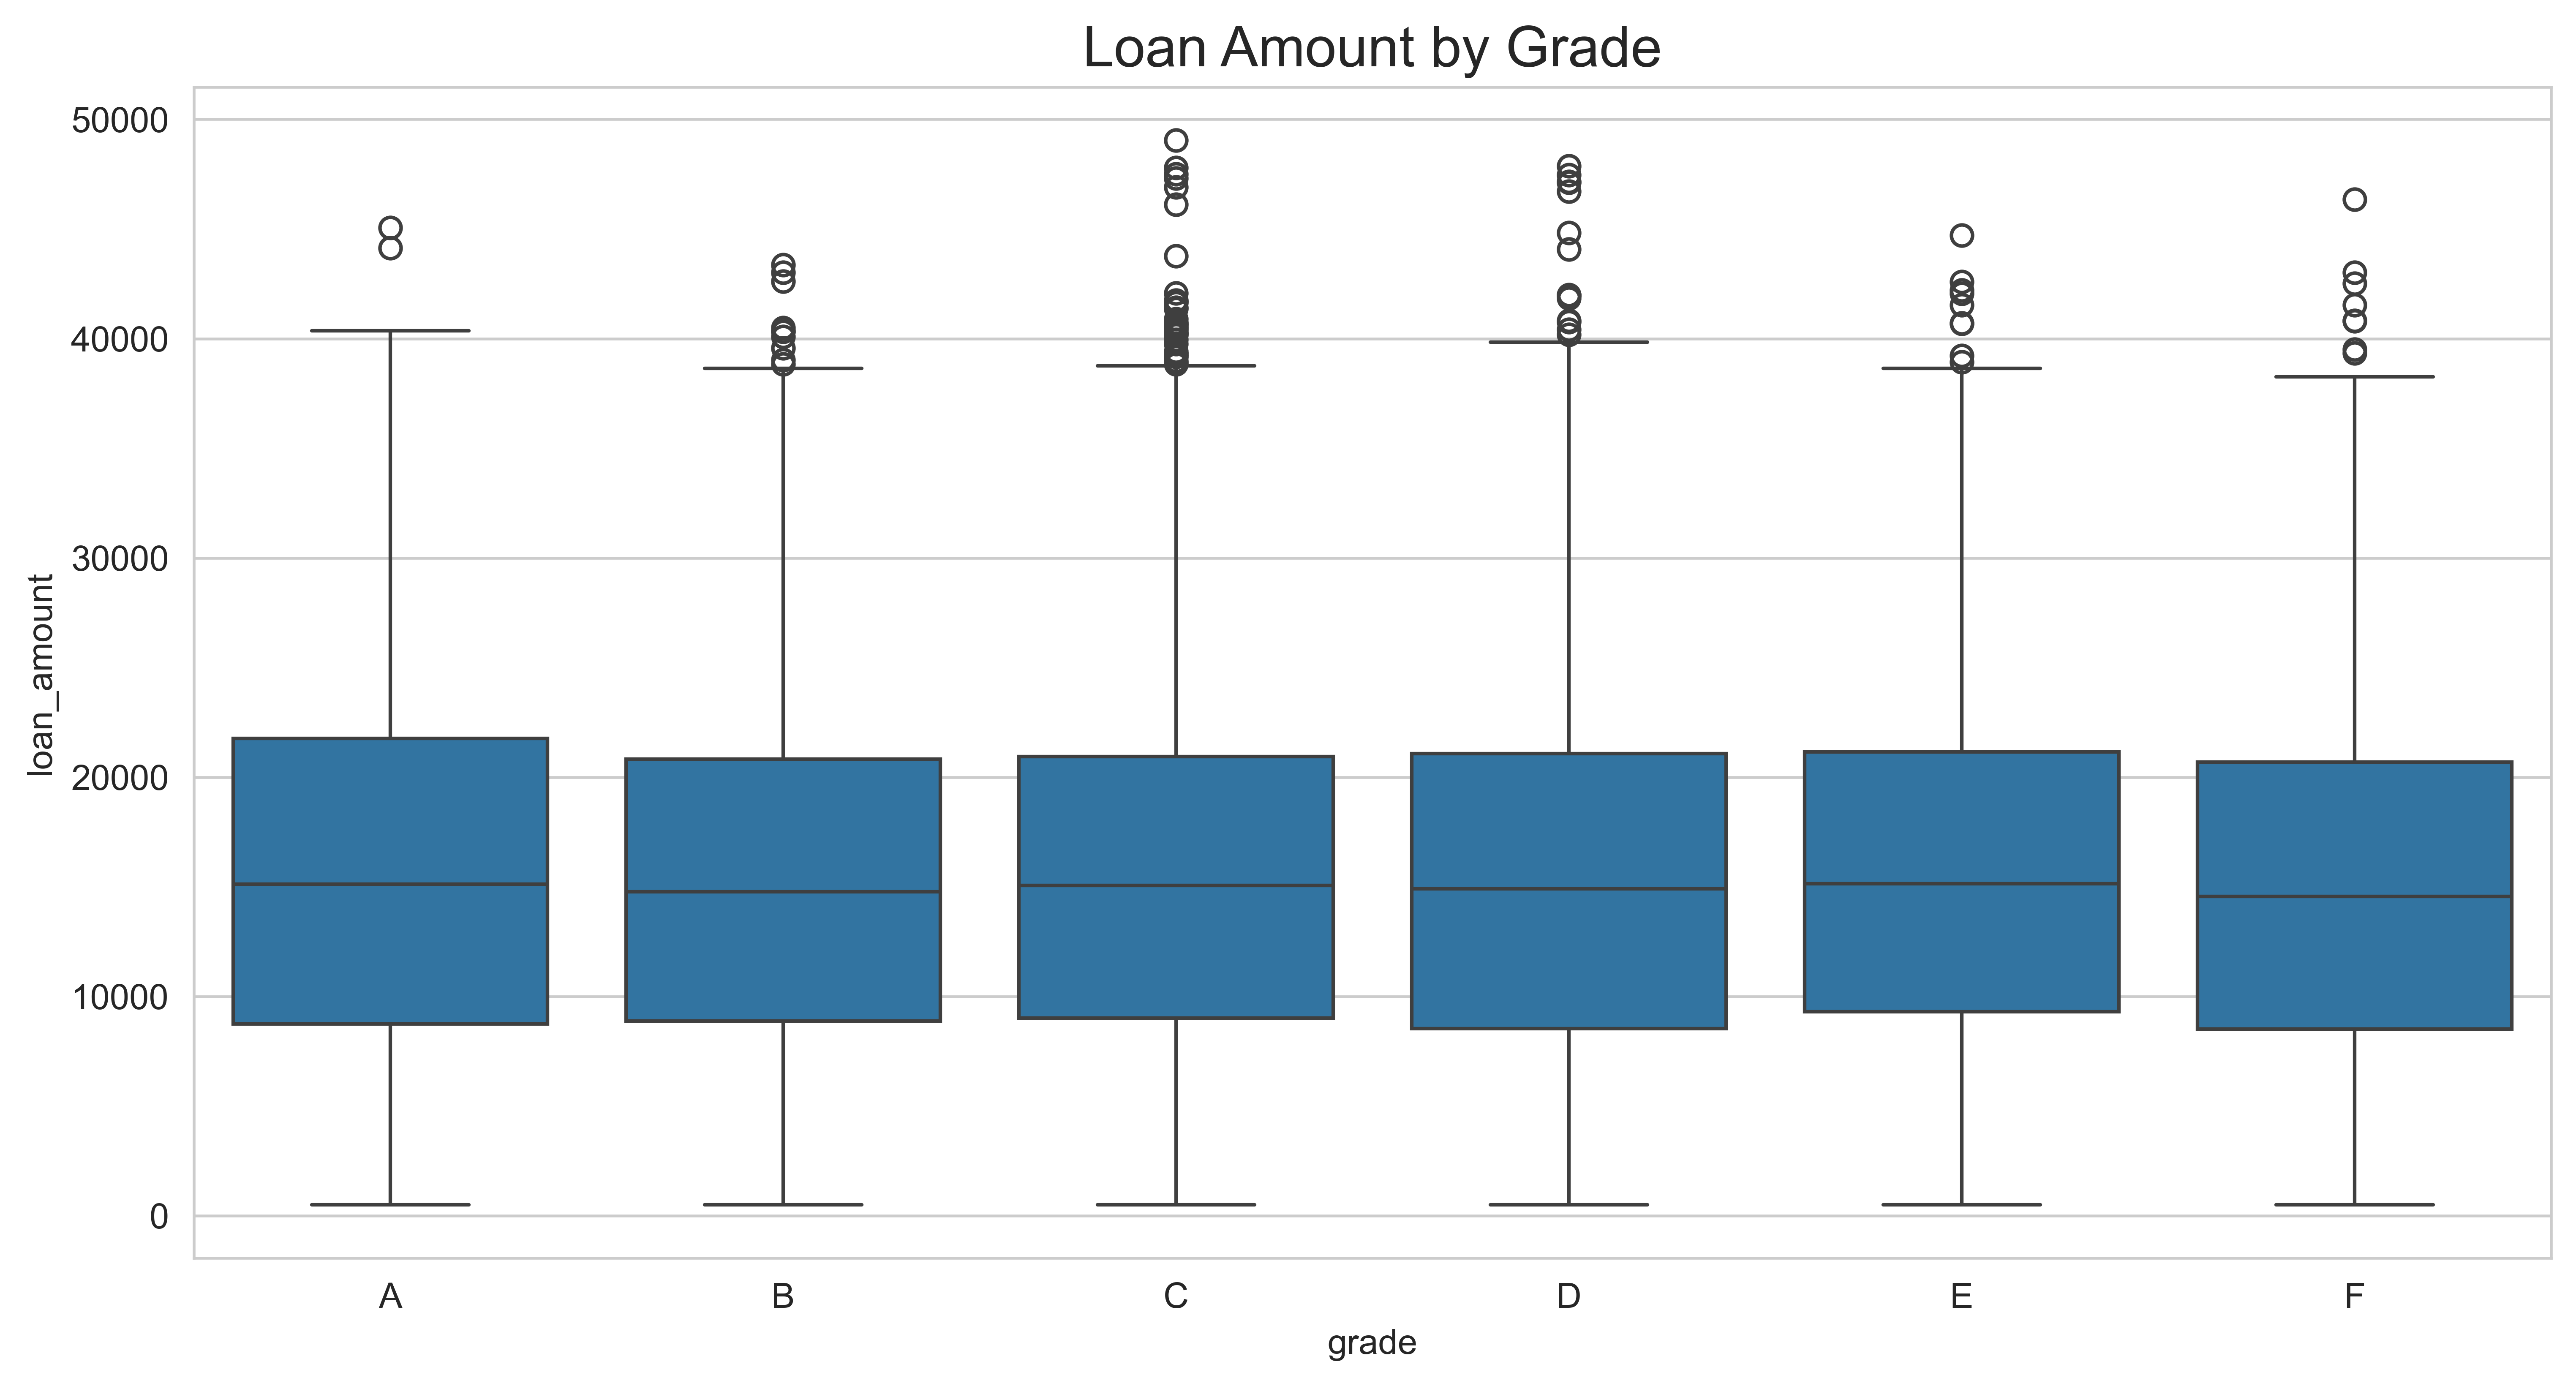
\includegraphics[width=0.8\textwidth]{png/loan_boxplot.png}
\caption{Box Plot by Grade - Loan Amount}
\end{figure}

\begin{figure}[H]
\centering
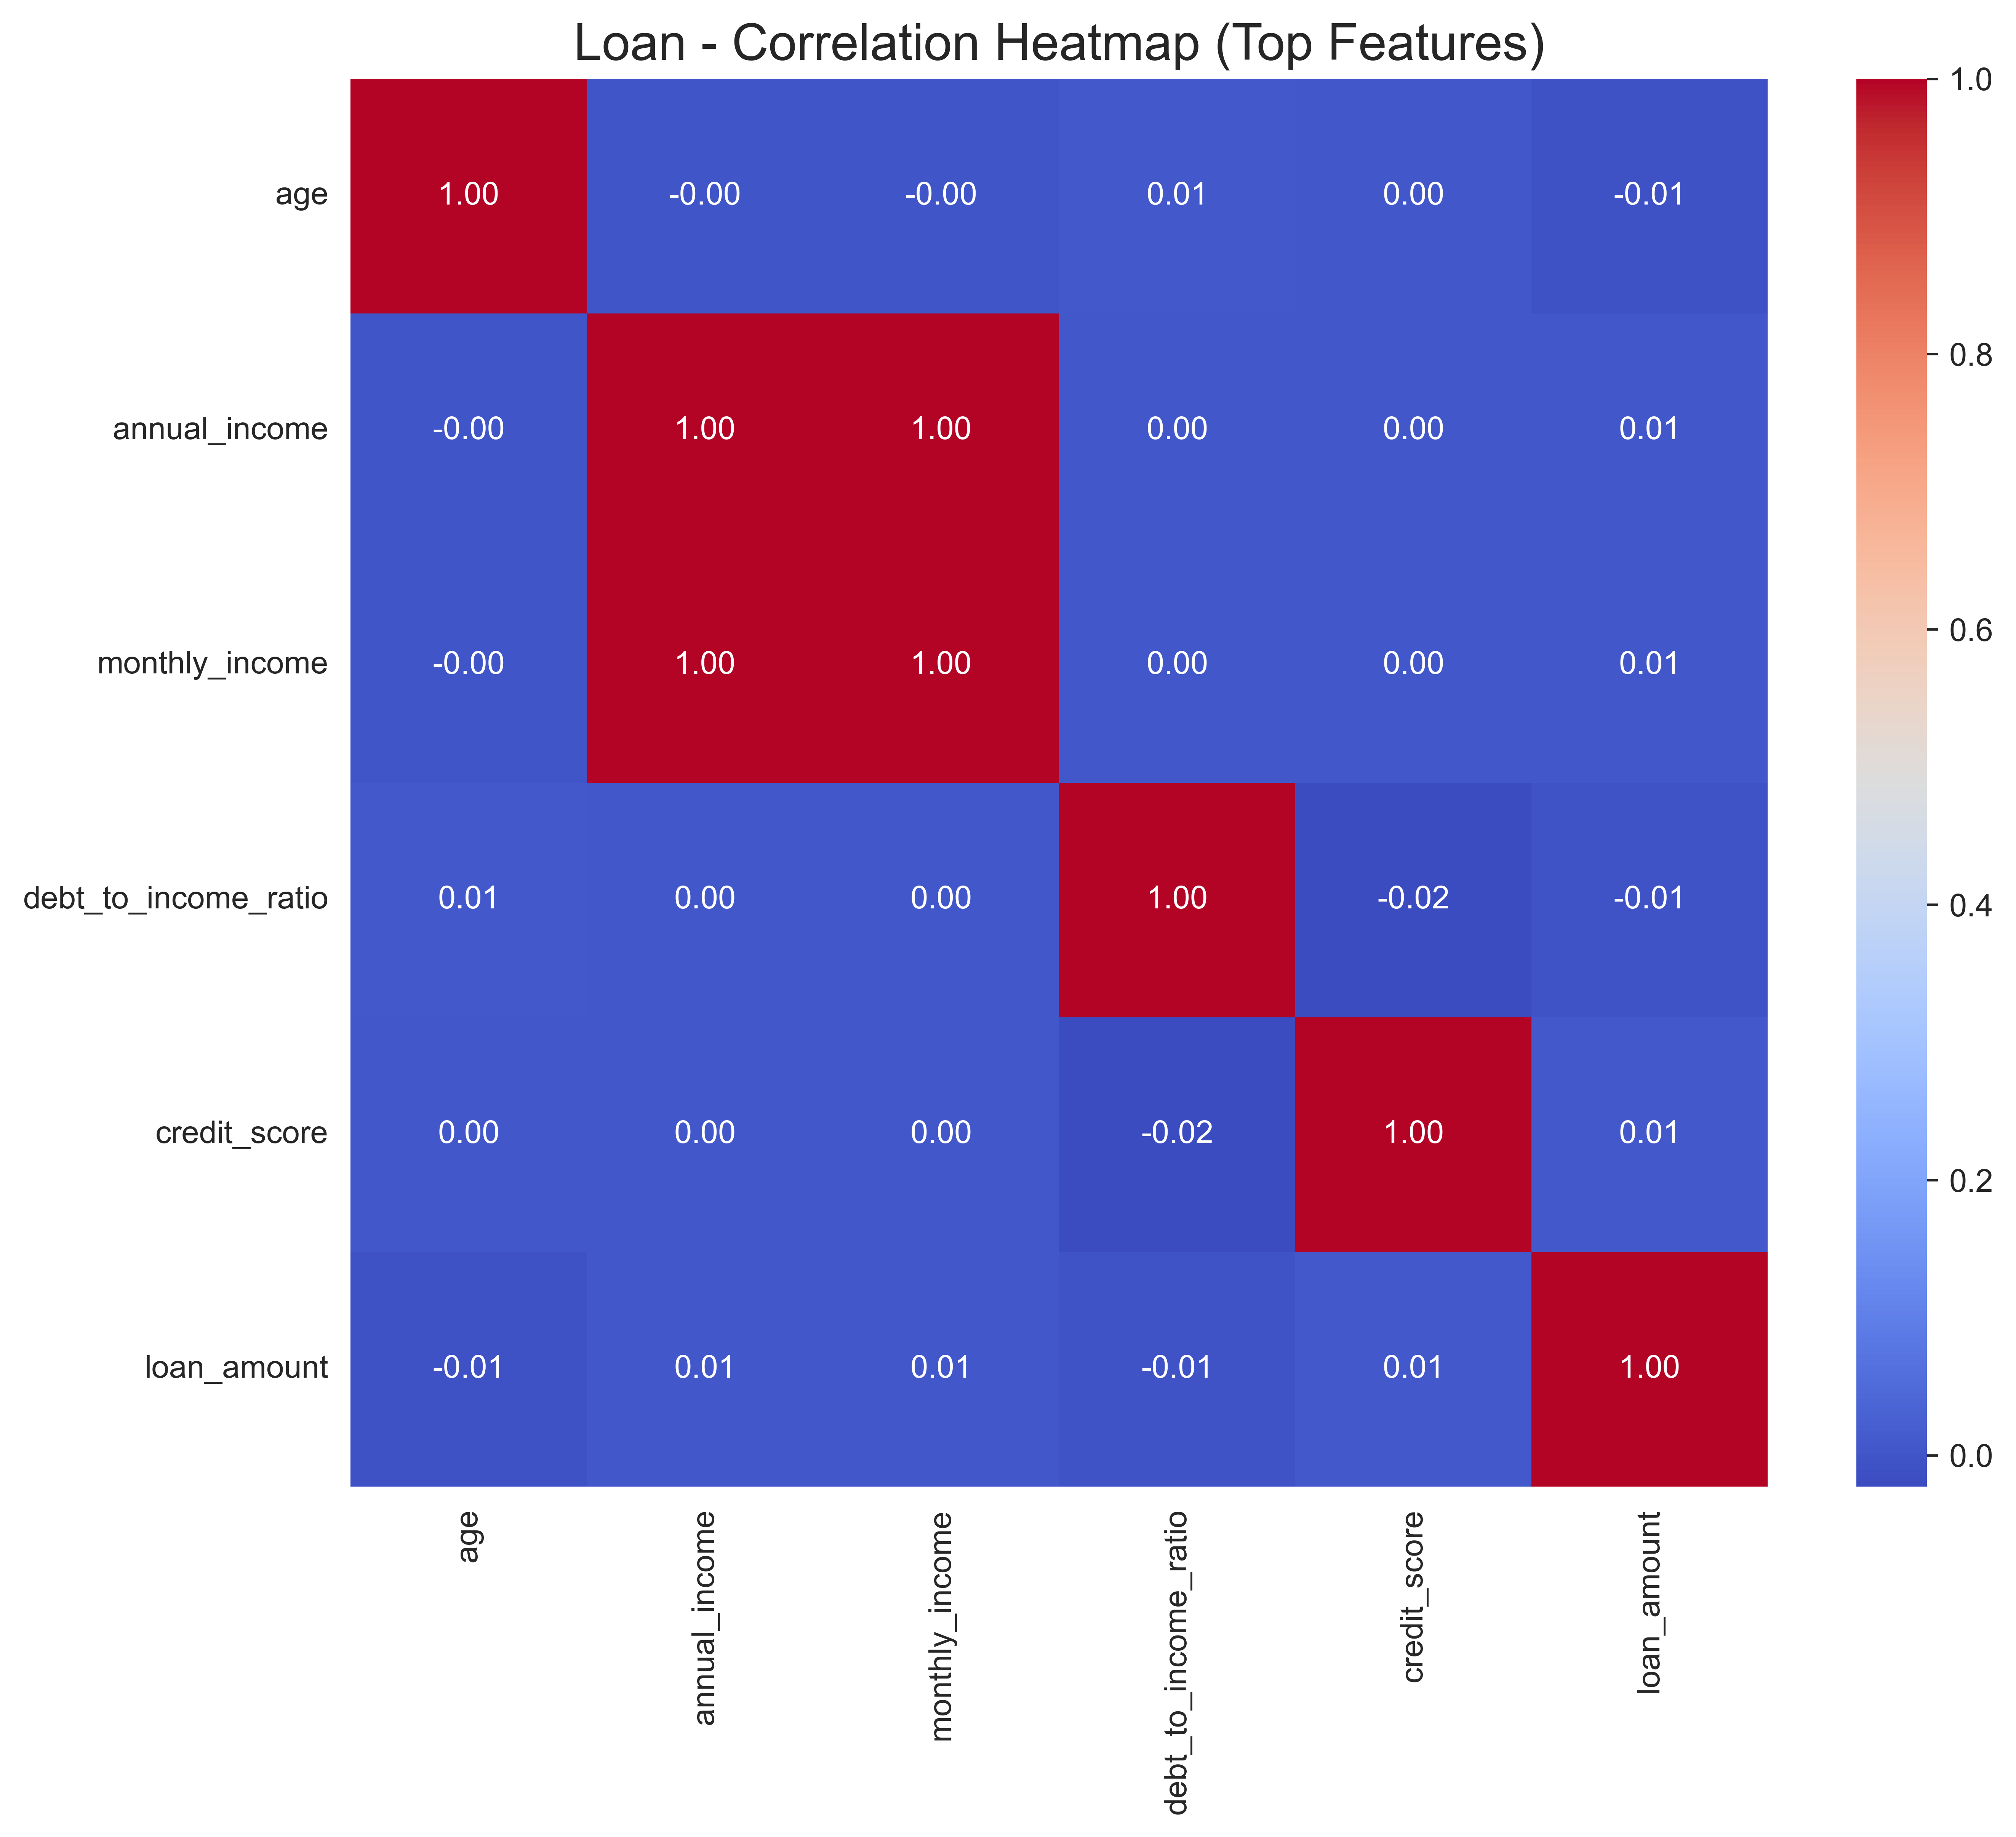
\includegraphics[width=0.8\textwidth]{png/loan_heatmap.png}
\caption{Feature Correlation Heatmap - Loan Amount}
\end{figure}

\begin{figure}[H]
\centering
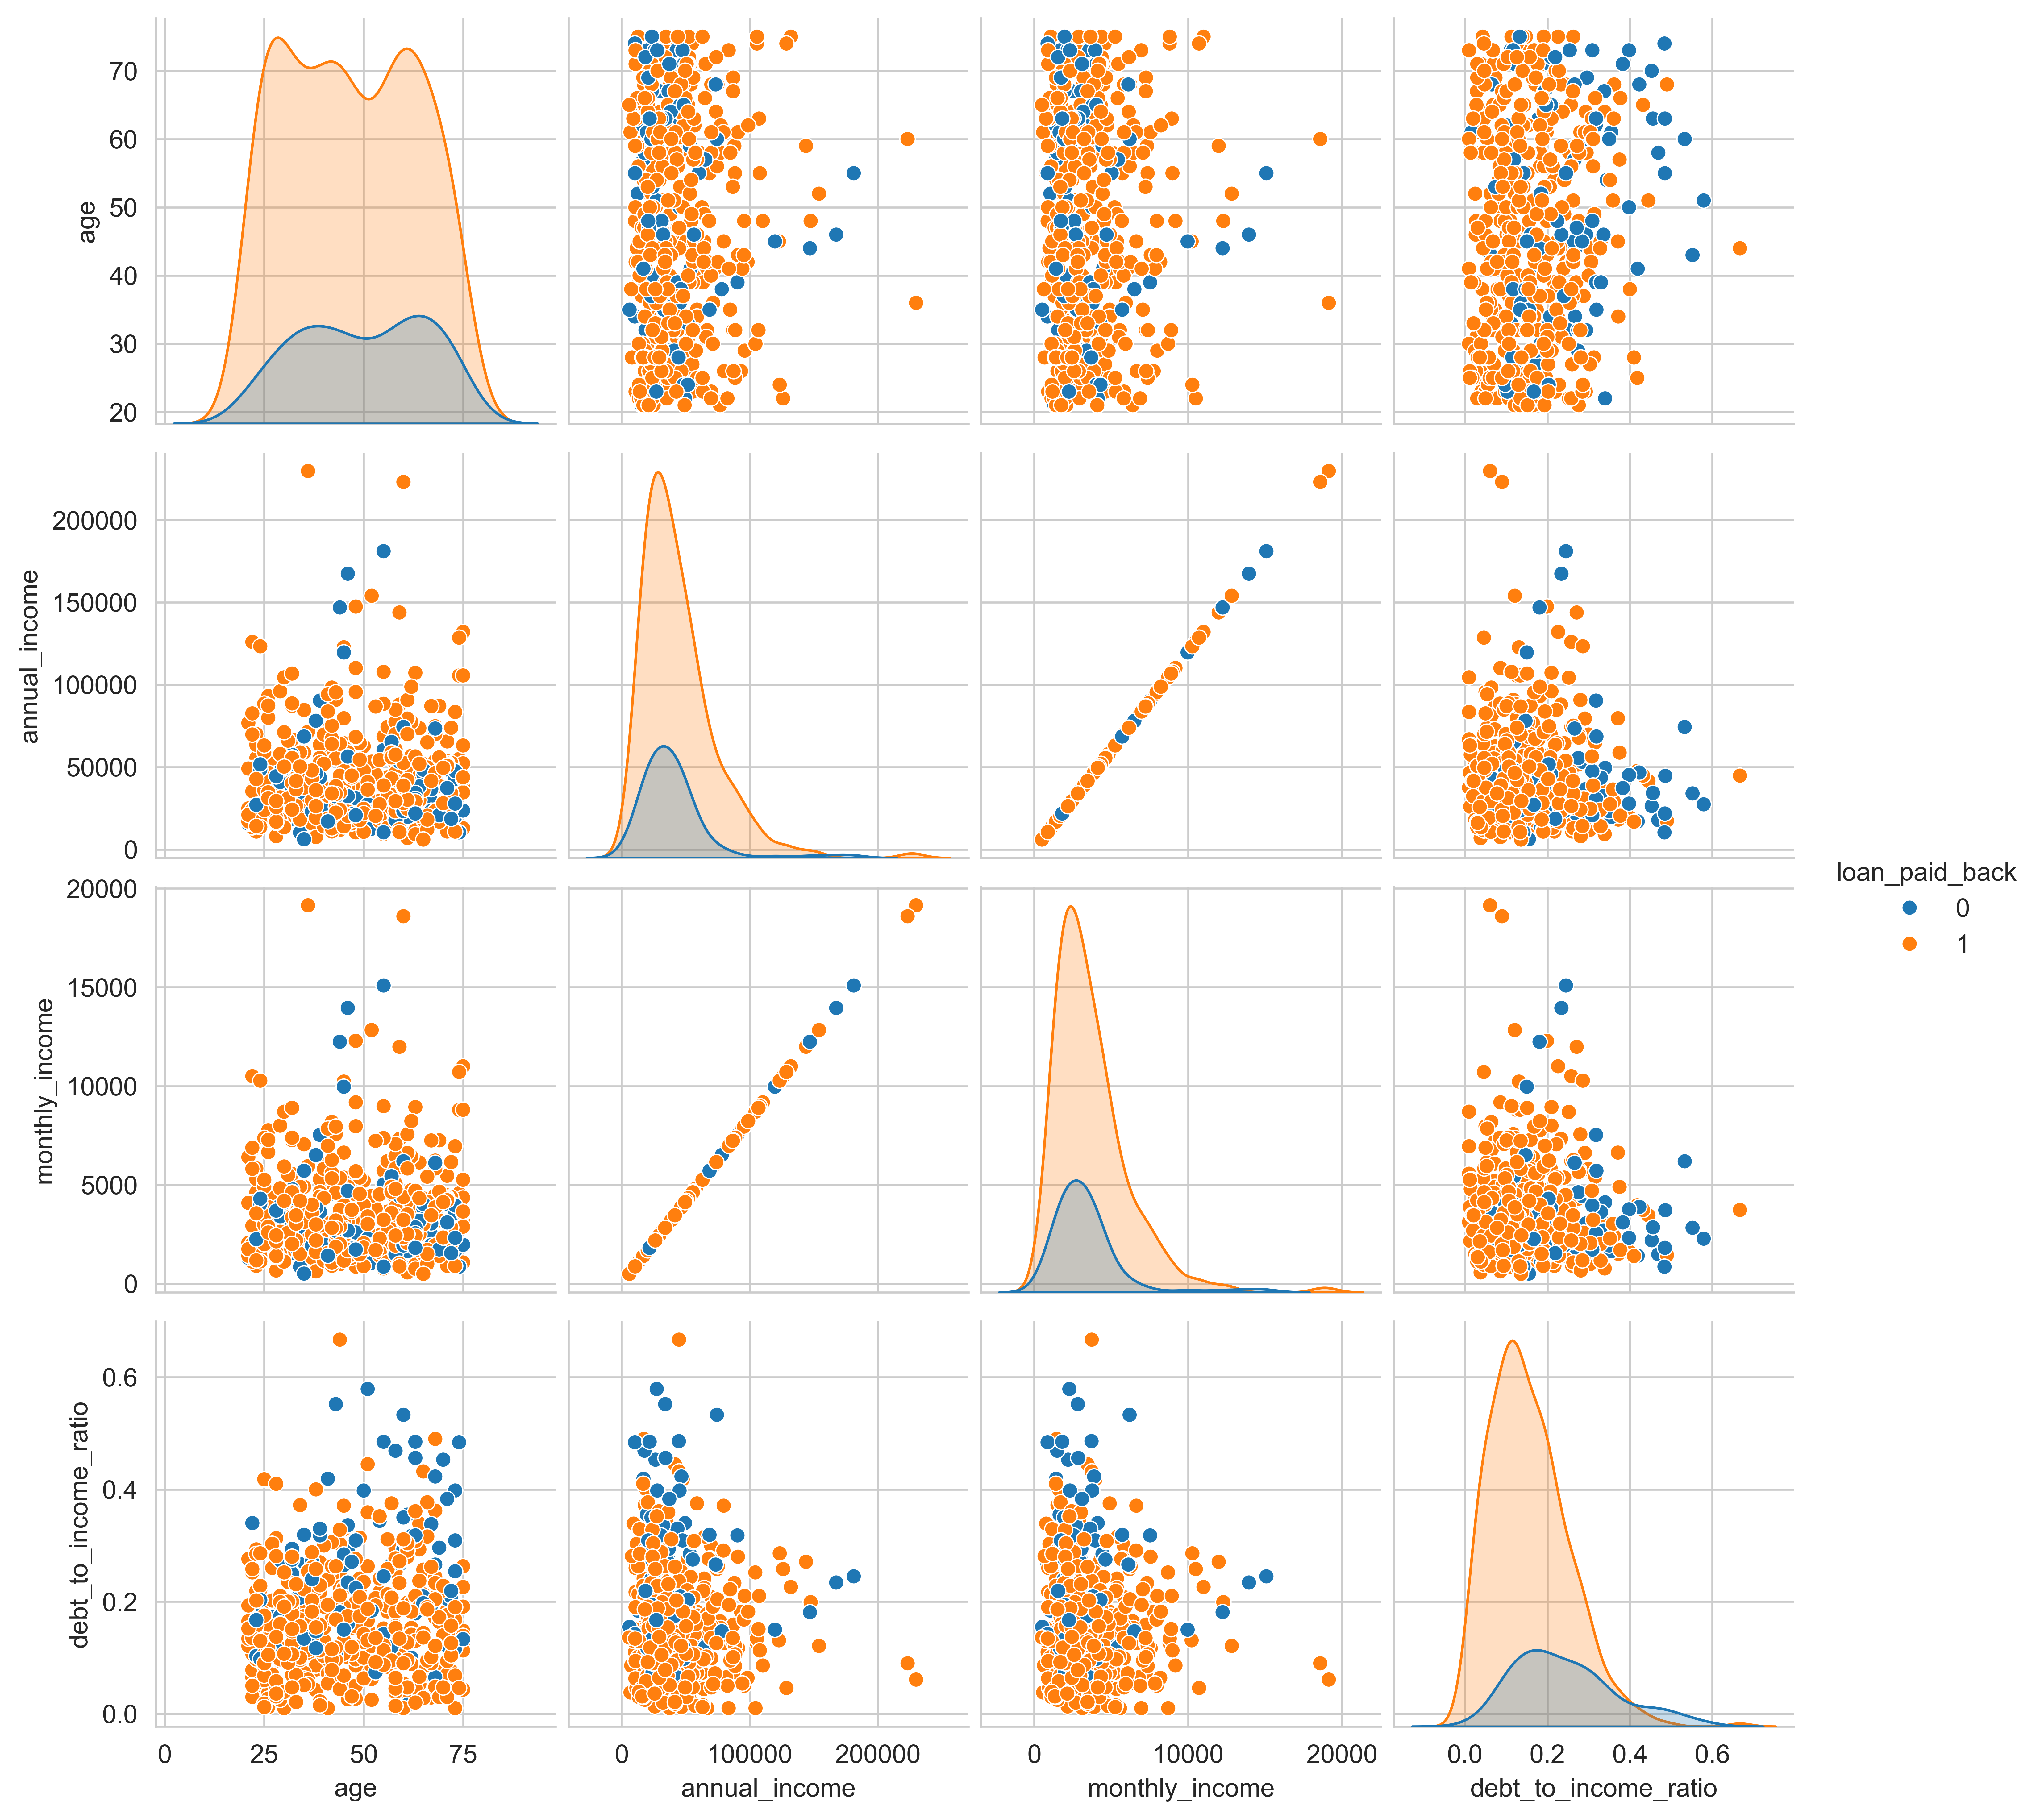
\includegraphics[width=0.85\textwidth]{png/loan_pairplot.png}
\caption{Pair Plot (Subset) - Loan Amount}
\end{figure}

\subsection*{3.3 Predicting Diabetes}

\begin{figure}[H]
\centering
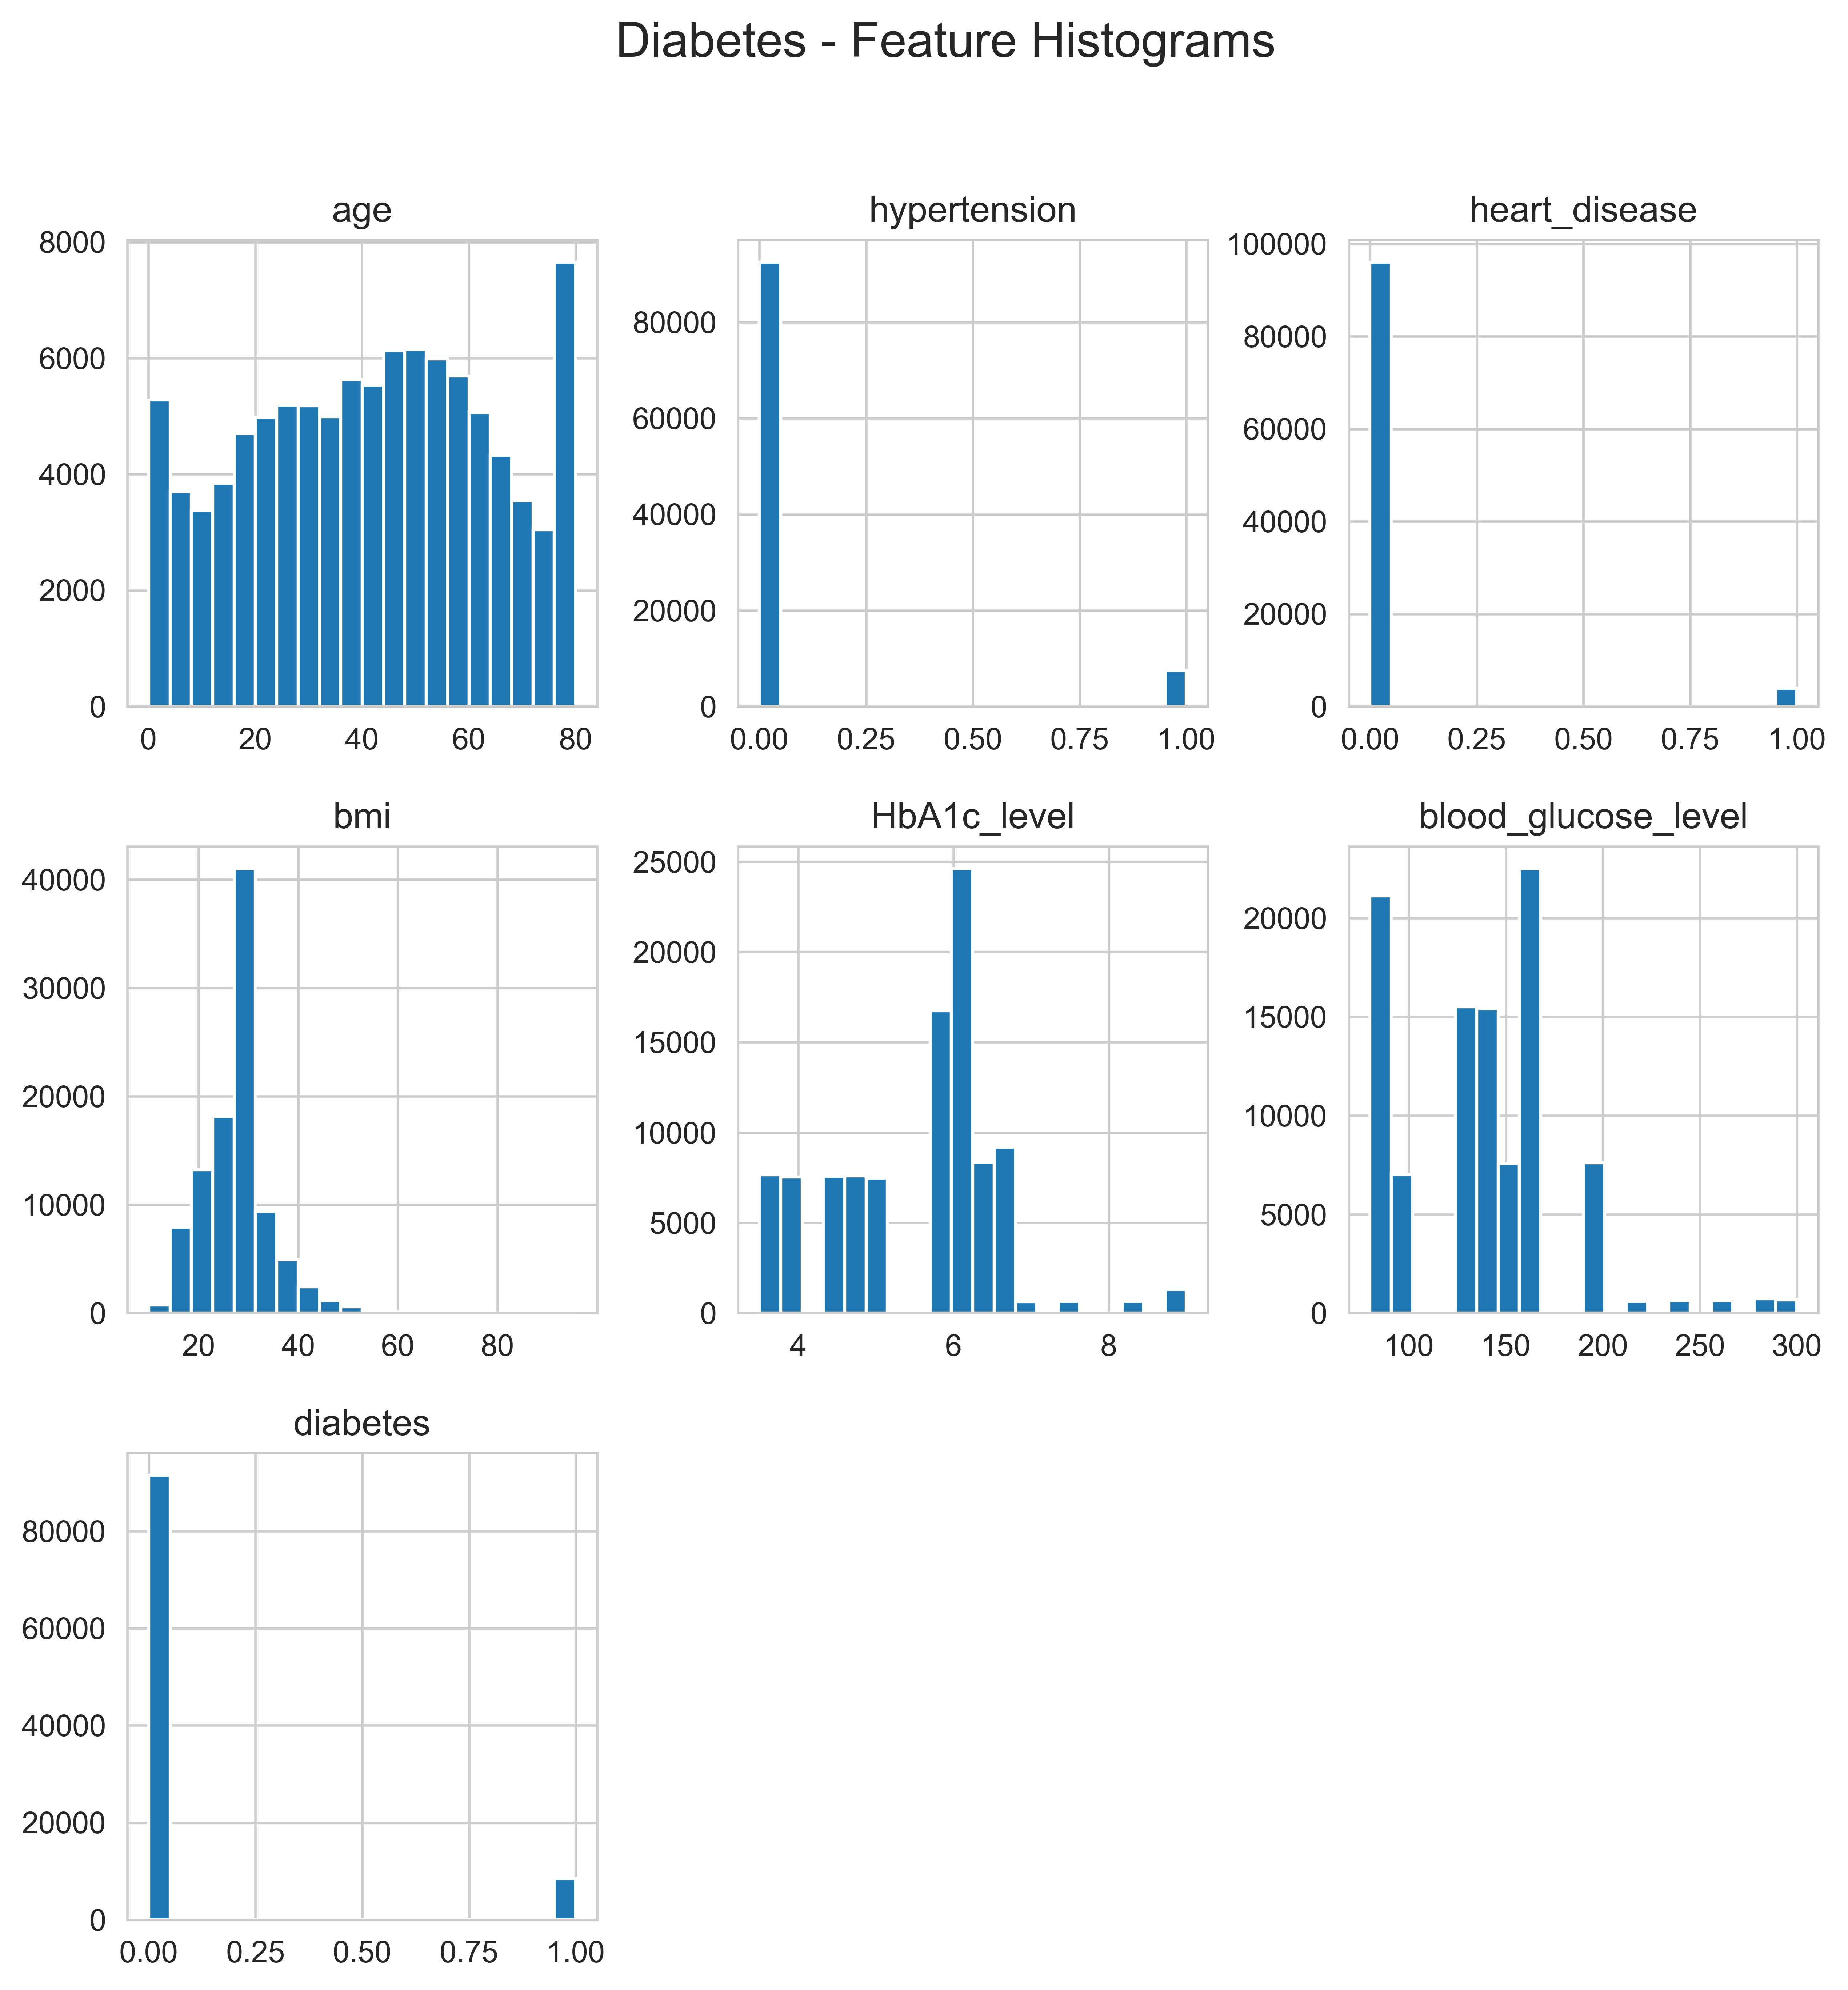
\includegraphics[width=0.85\textwidth]{png/diabetes_histograms.png}
\caption{Feature Histograms - Diabetes Dataset}
\end{figure}

\begin{figure}[H]
\centering
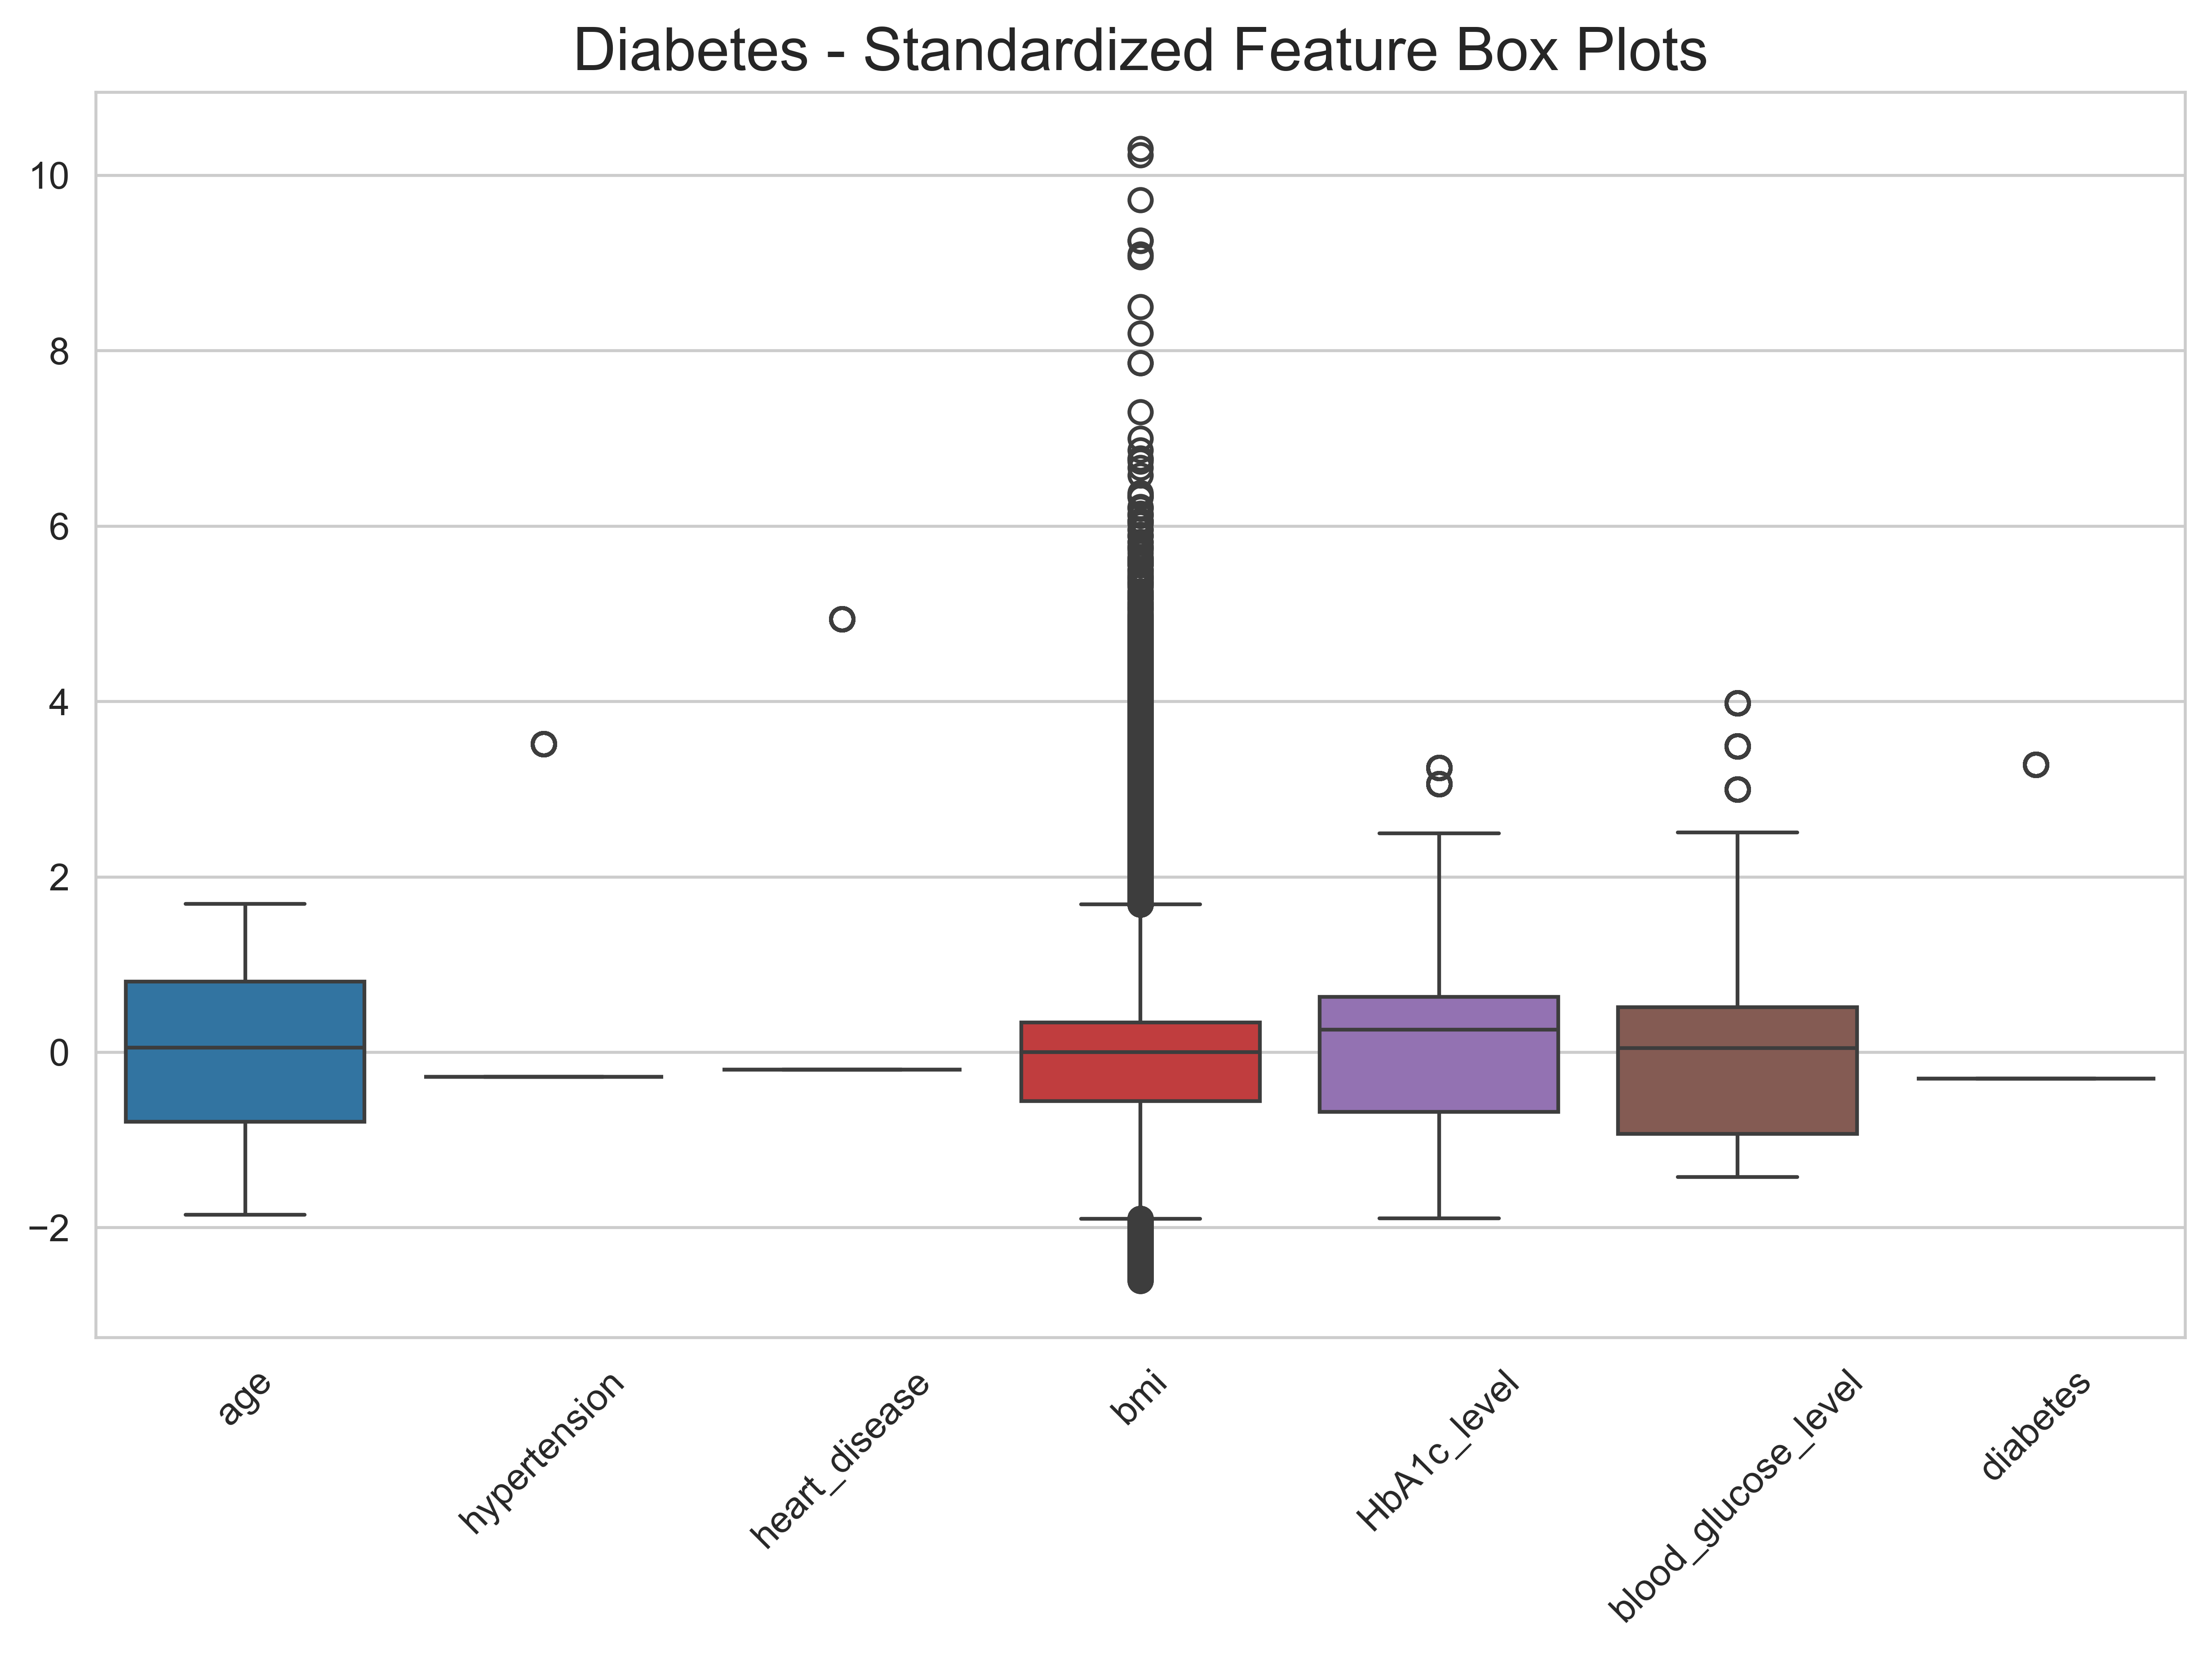
\includegraphics[width=0.8\textwidth]{png/diabetes_boxplot.png}
\caption{Standardized Box Plots - Diabetes Dataset}
\end{figure}

\begin{figure}[H]
\centering
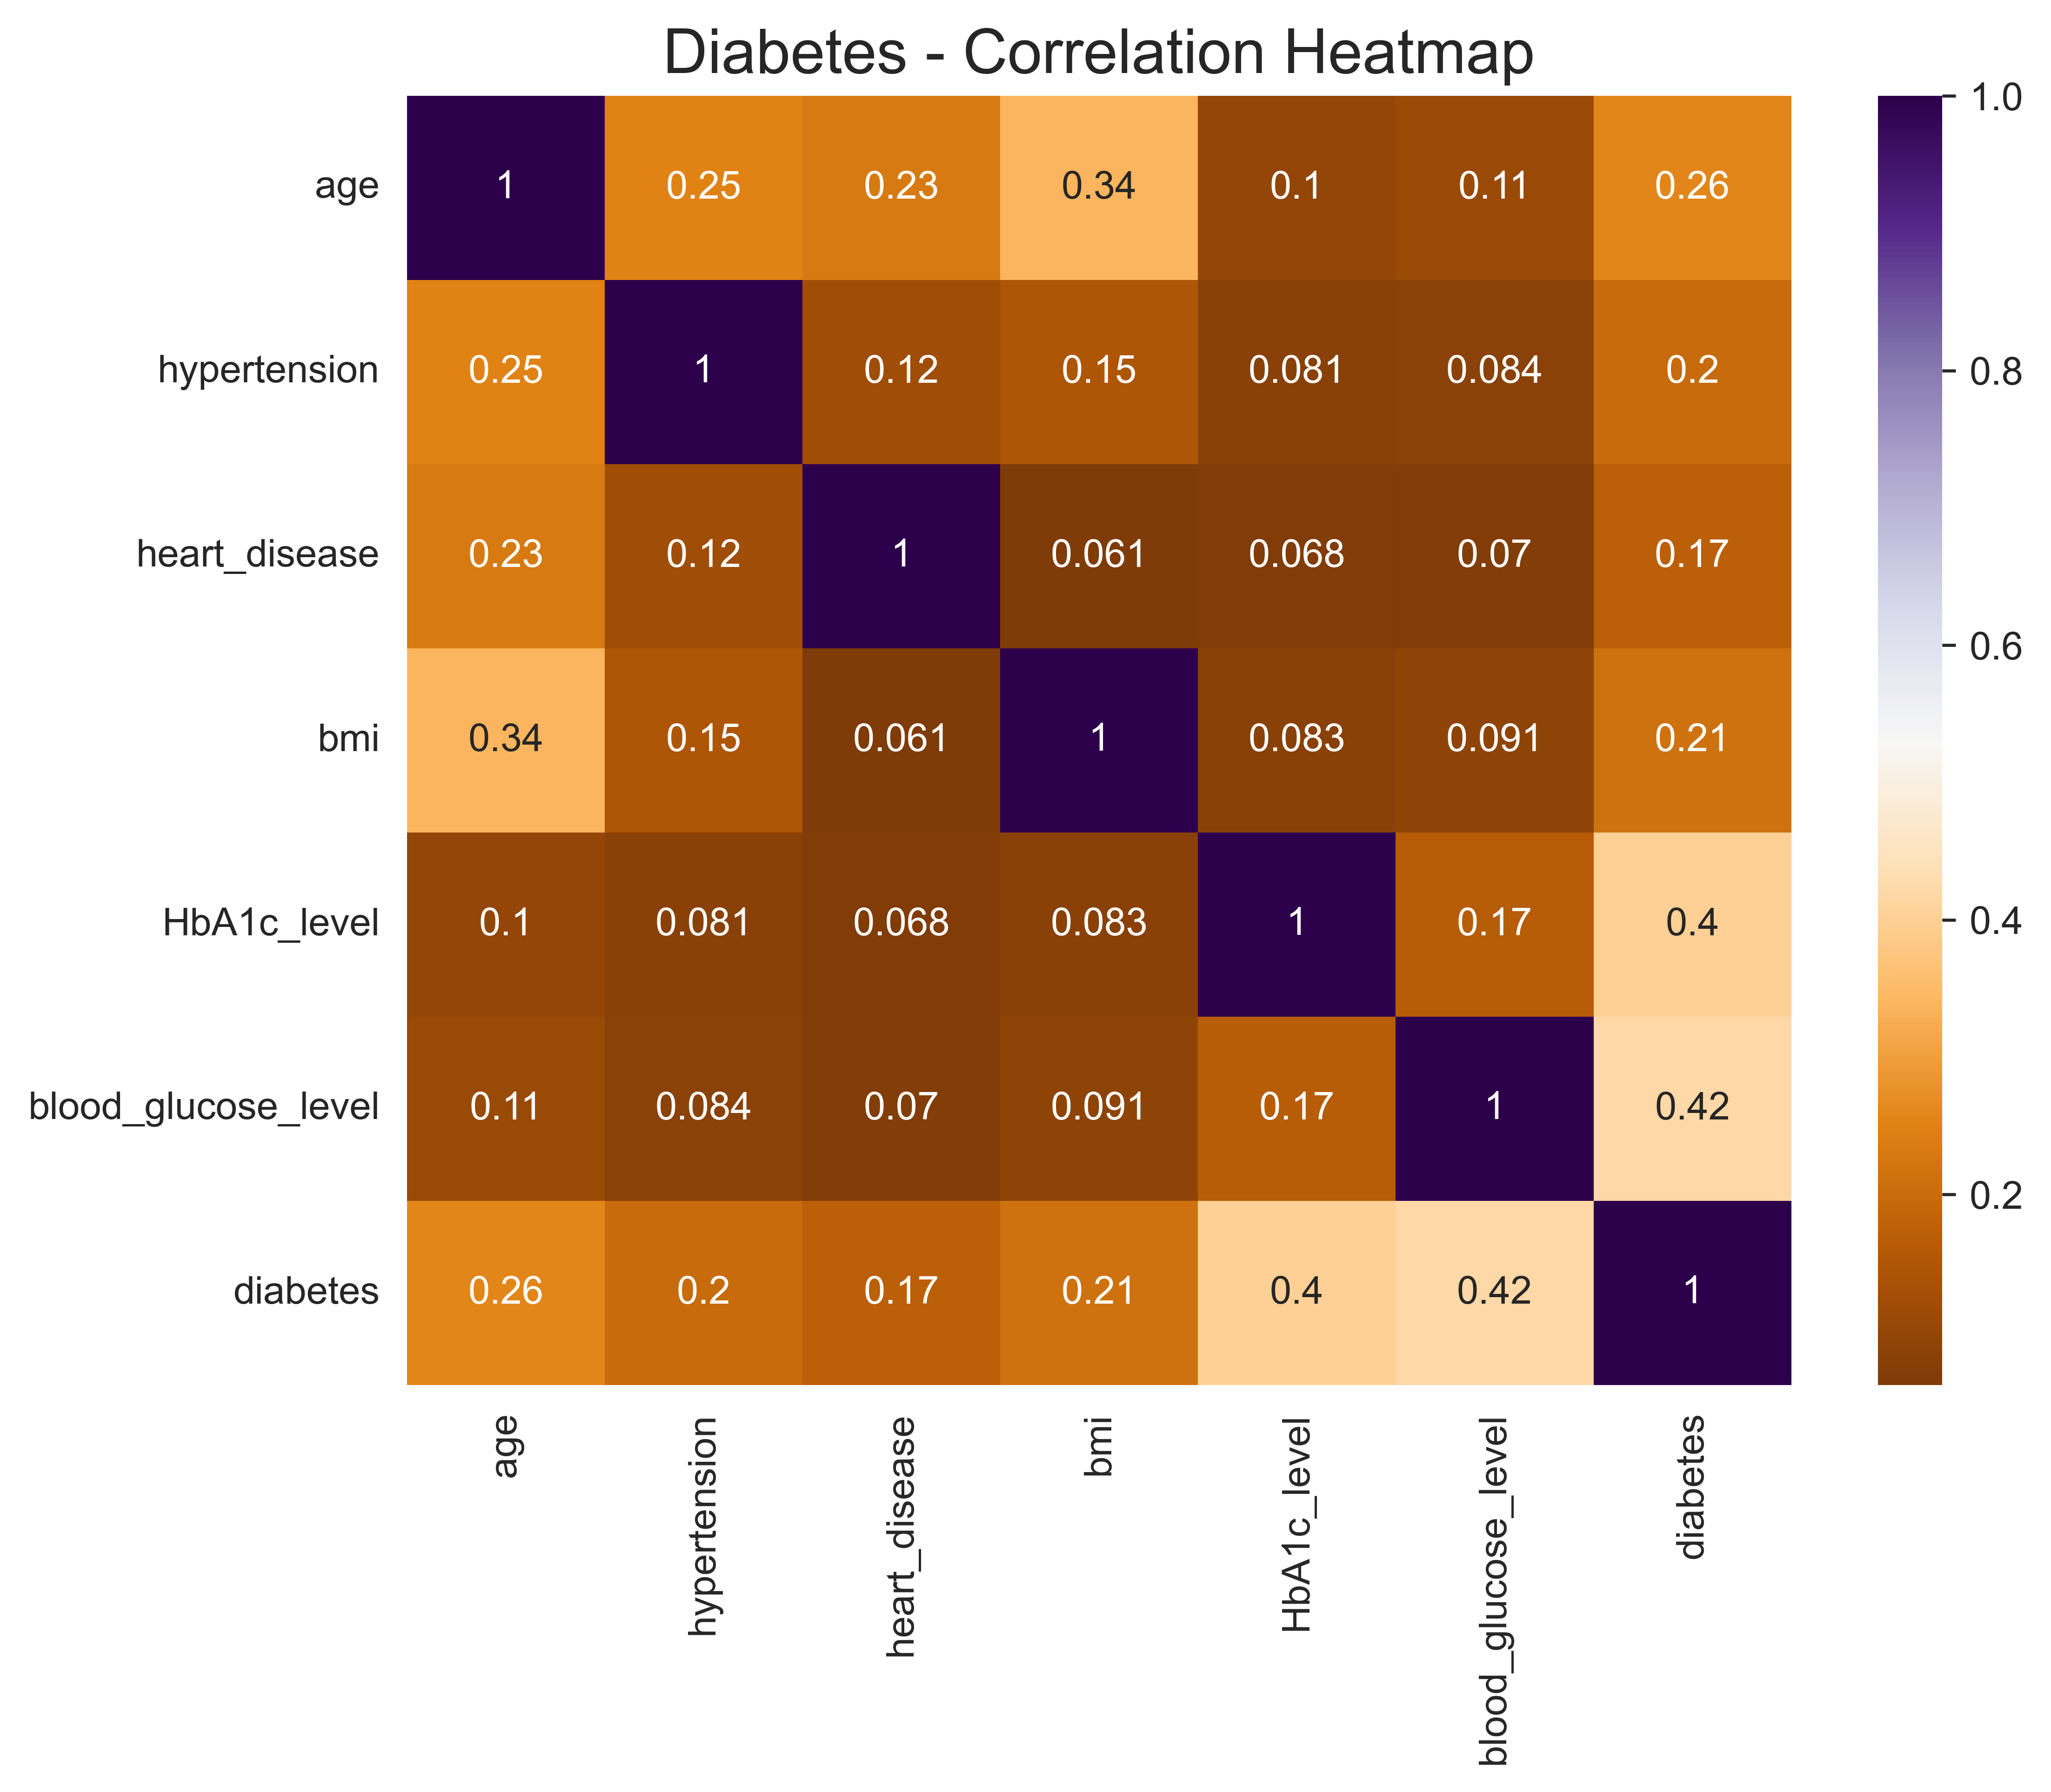
\includegraphics[width=0.7\textwidth]{png/diabetes_heatmap.png}
\caption{Correlation Heatmap - Diabetes Dataset}
\end{figure}

\begin{figure}[H]
\centering
\includegraphics[width=0.85\textwidth]{png/diabetes_pairplot.png}
\caption{Pair Plot Classification - Diabetes Dataset}
\end{figure}

\subsection*{3.4 Classification of Email Spam}

\begin{figure}[H]
\centering
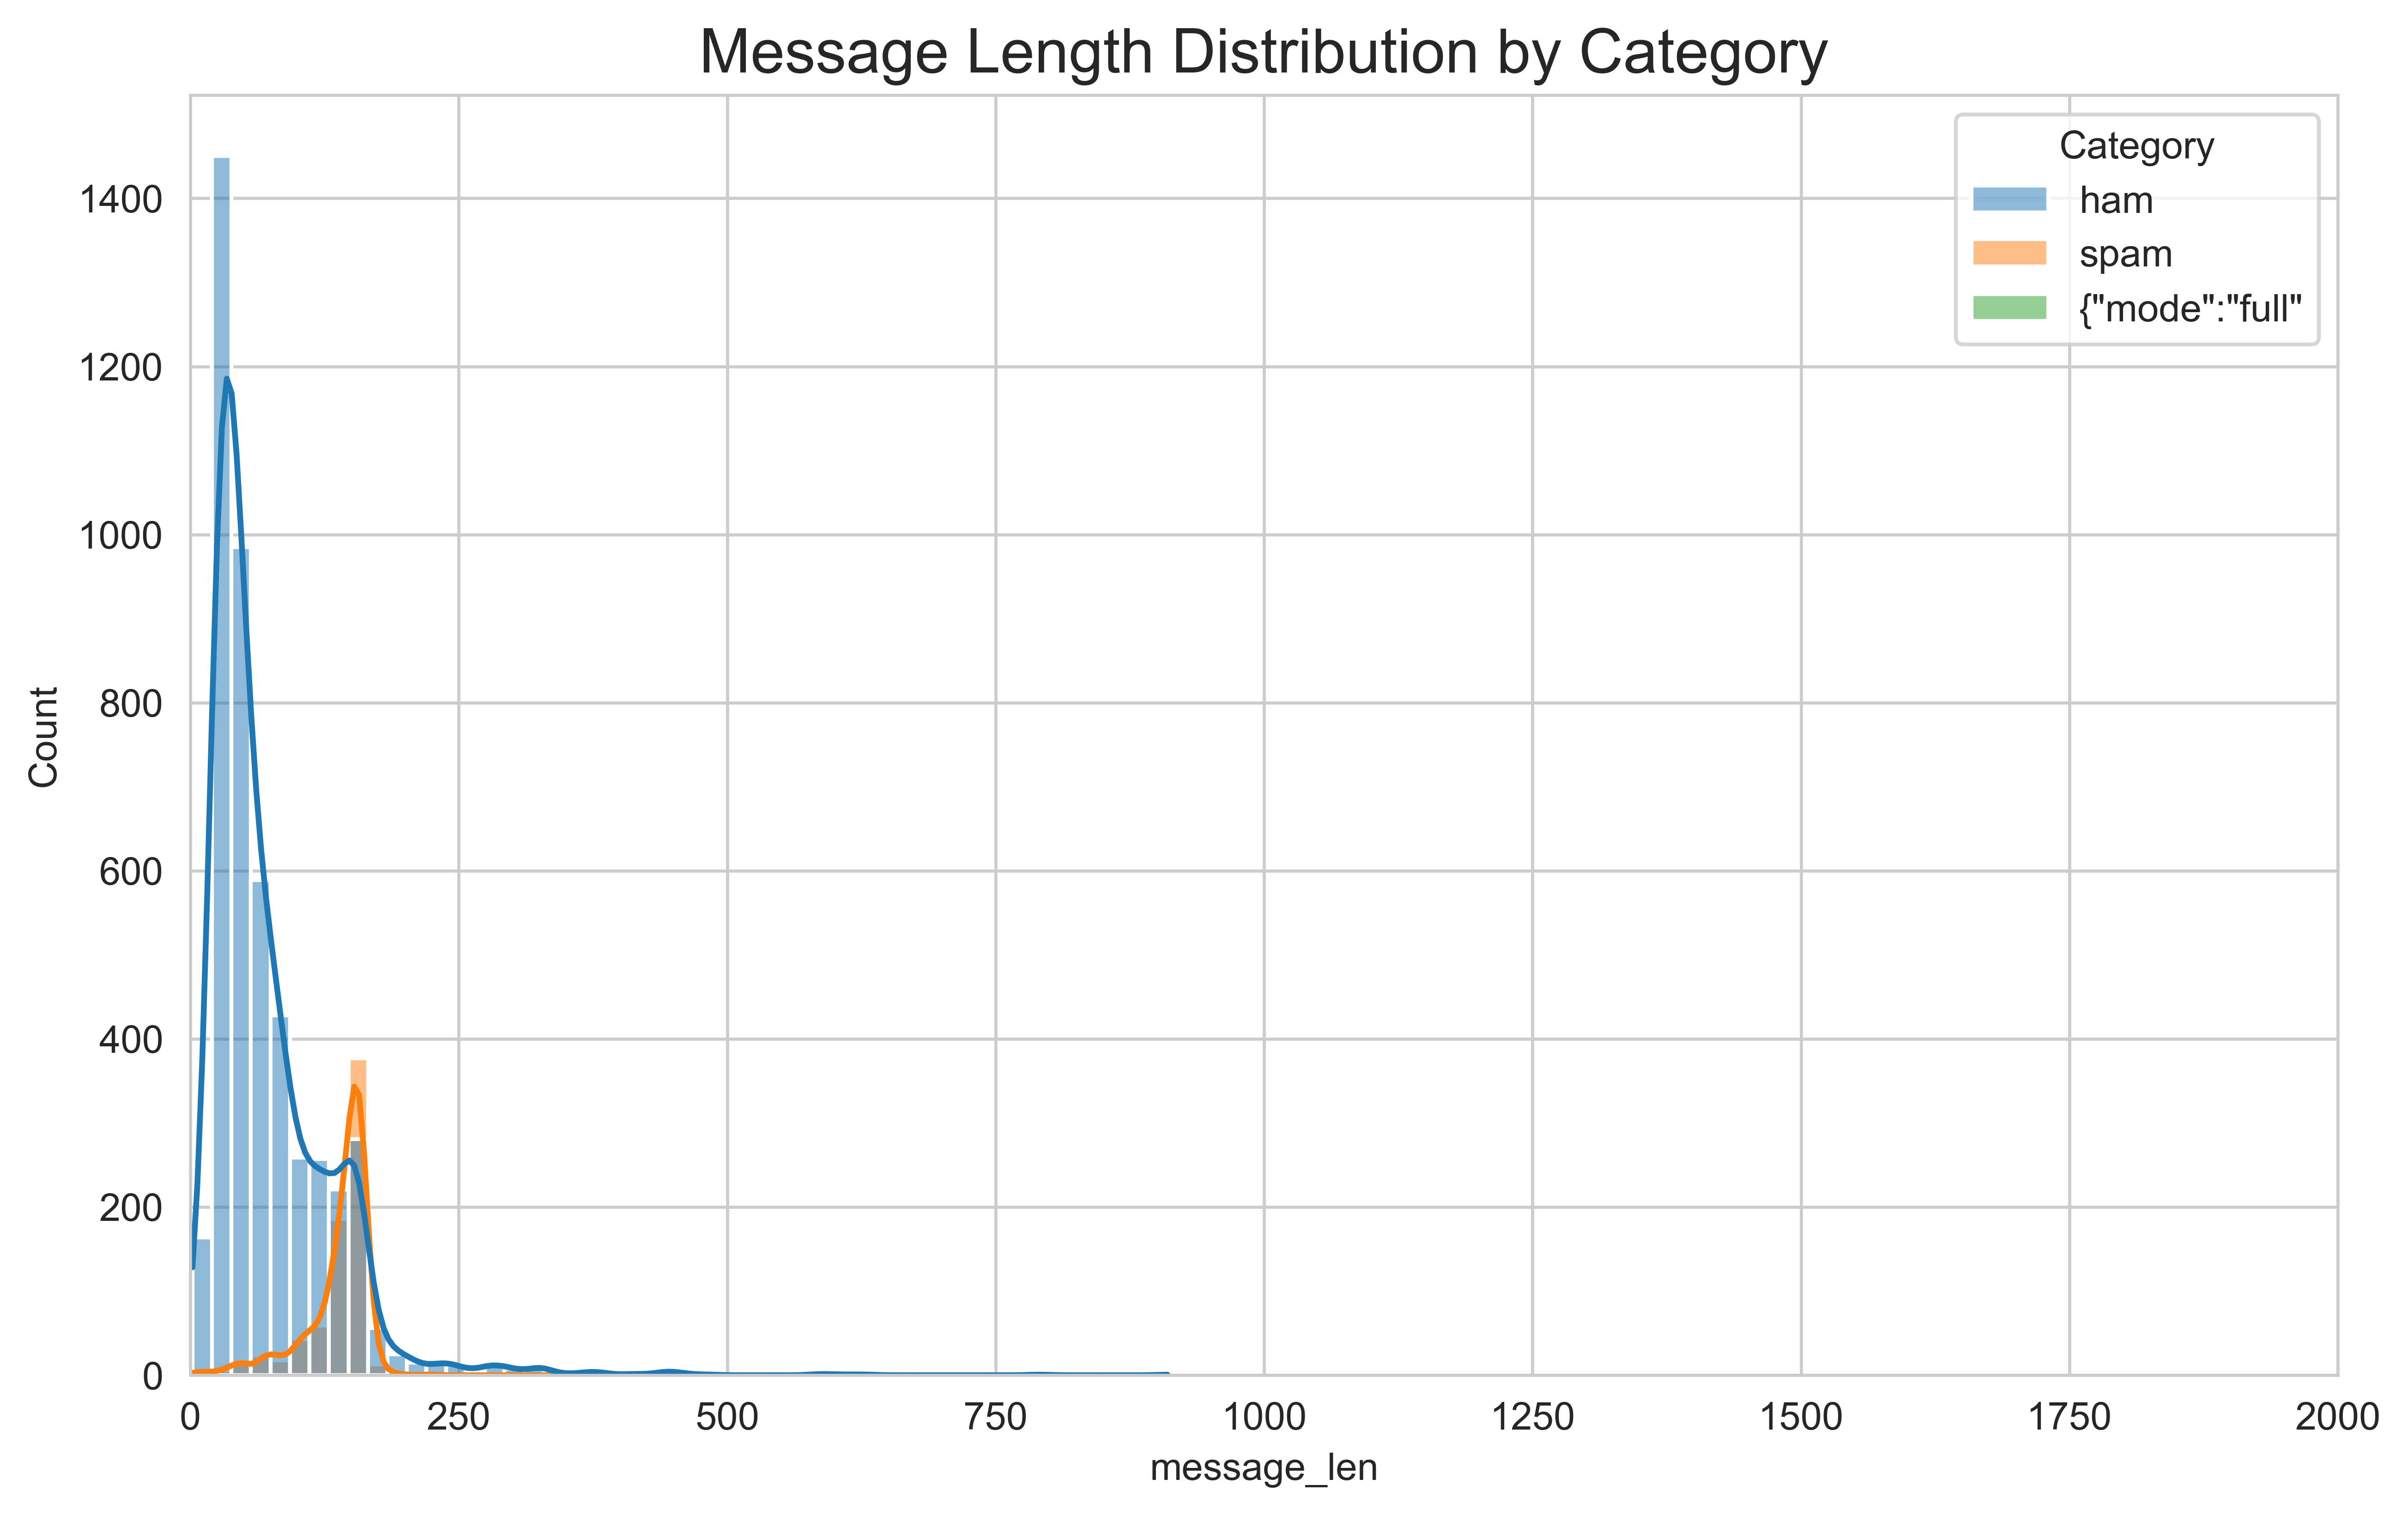
\includegraphics[width=0.8\textwidth]{png/spam_hist_length.png}
\caption{Message Length Distribution - Email Spam}
\end{figure}

\begin{figure}[H]
\centering
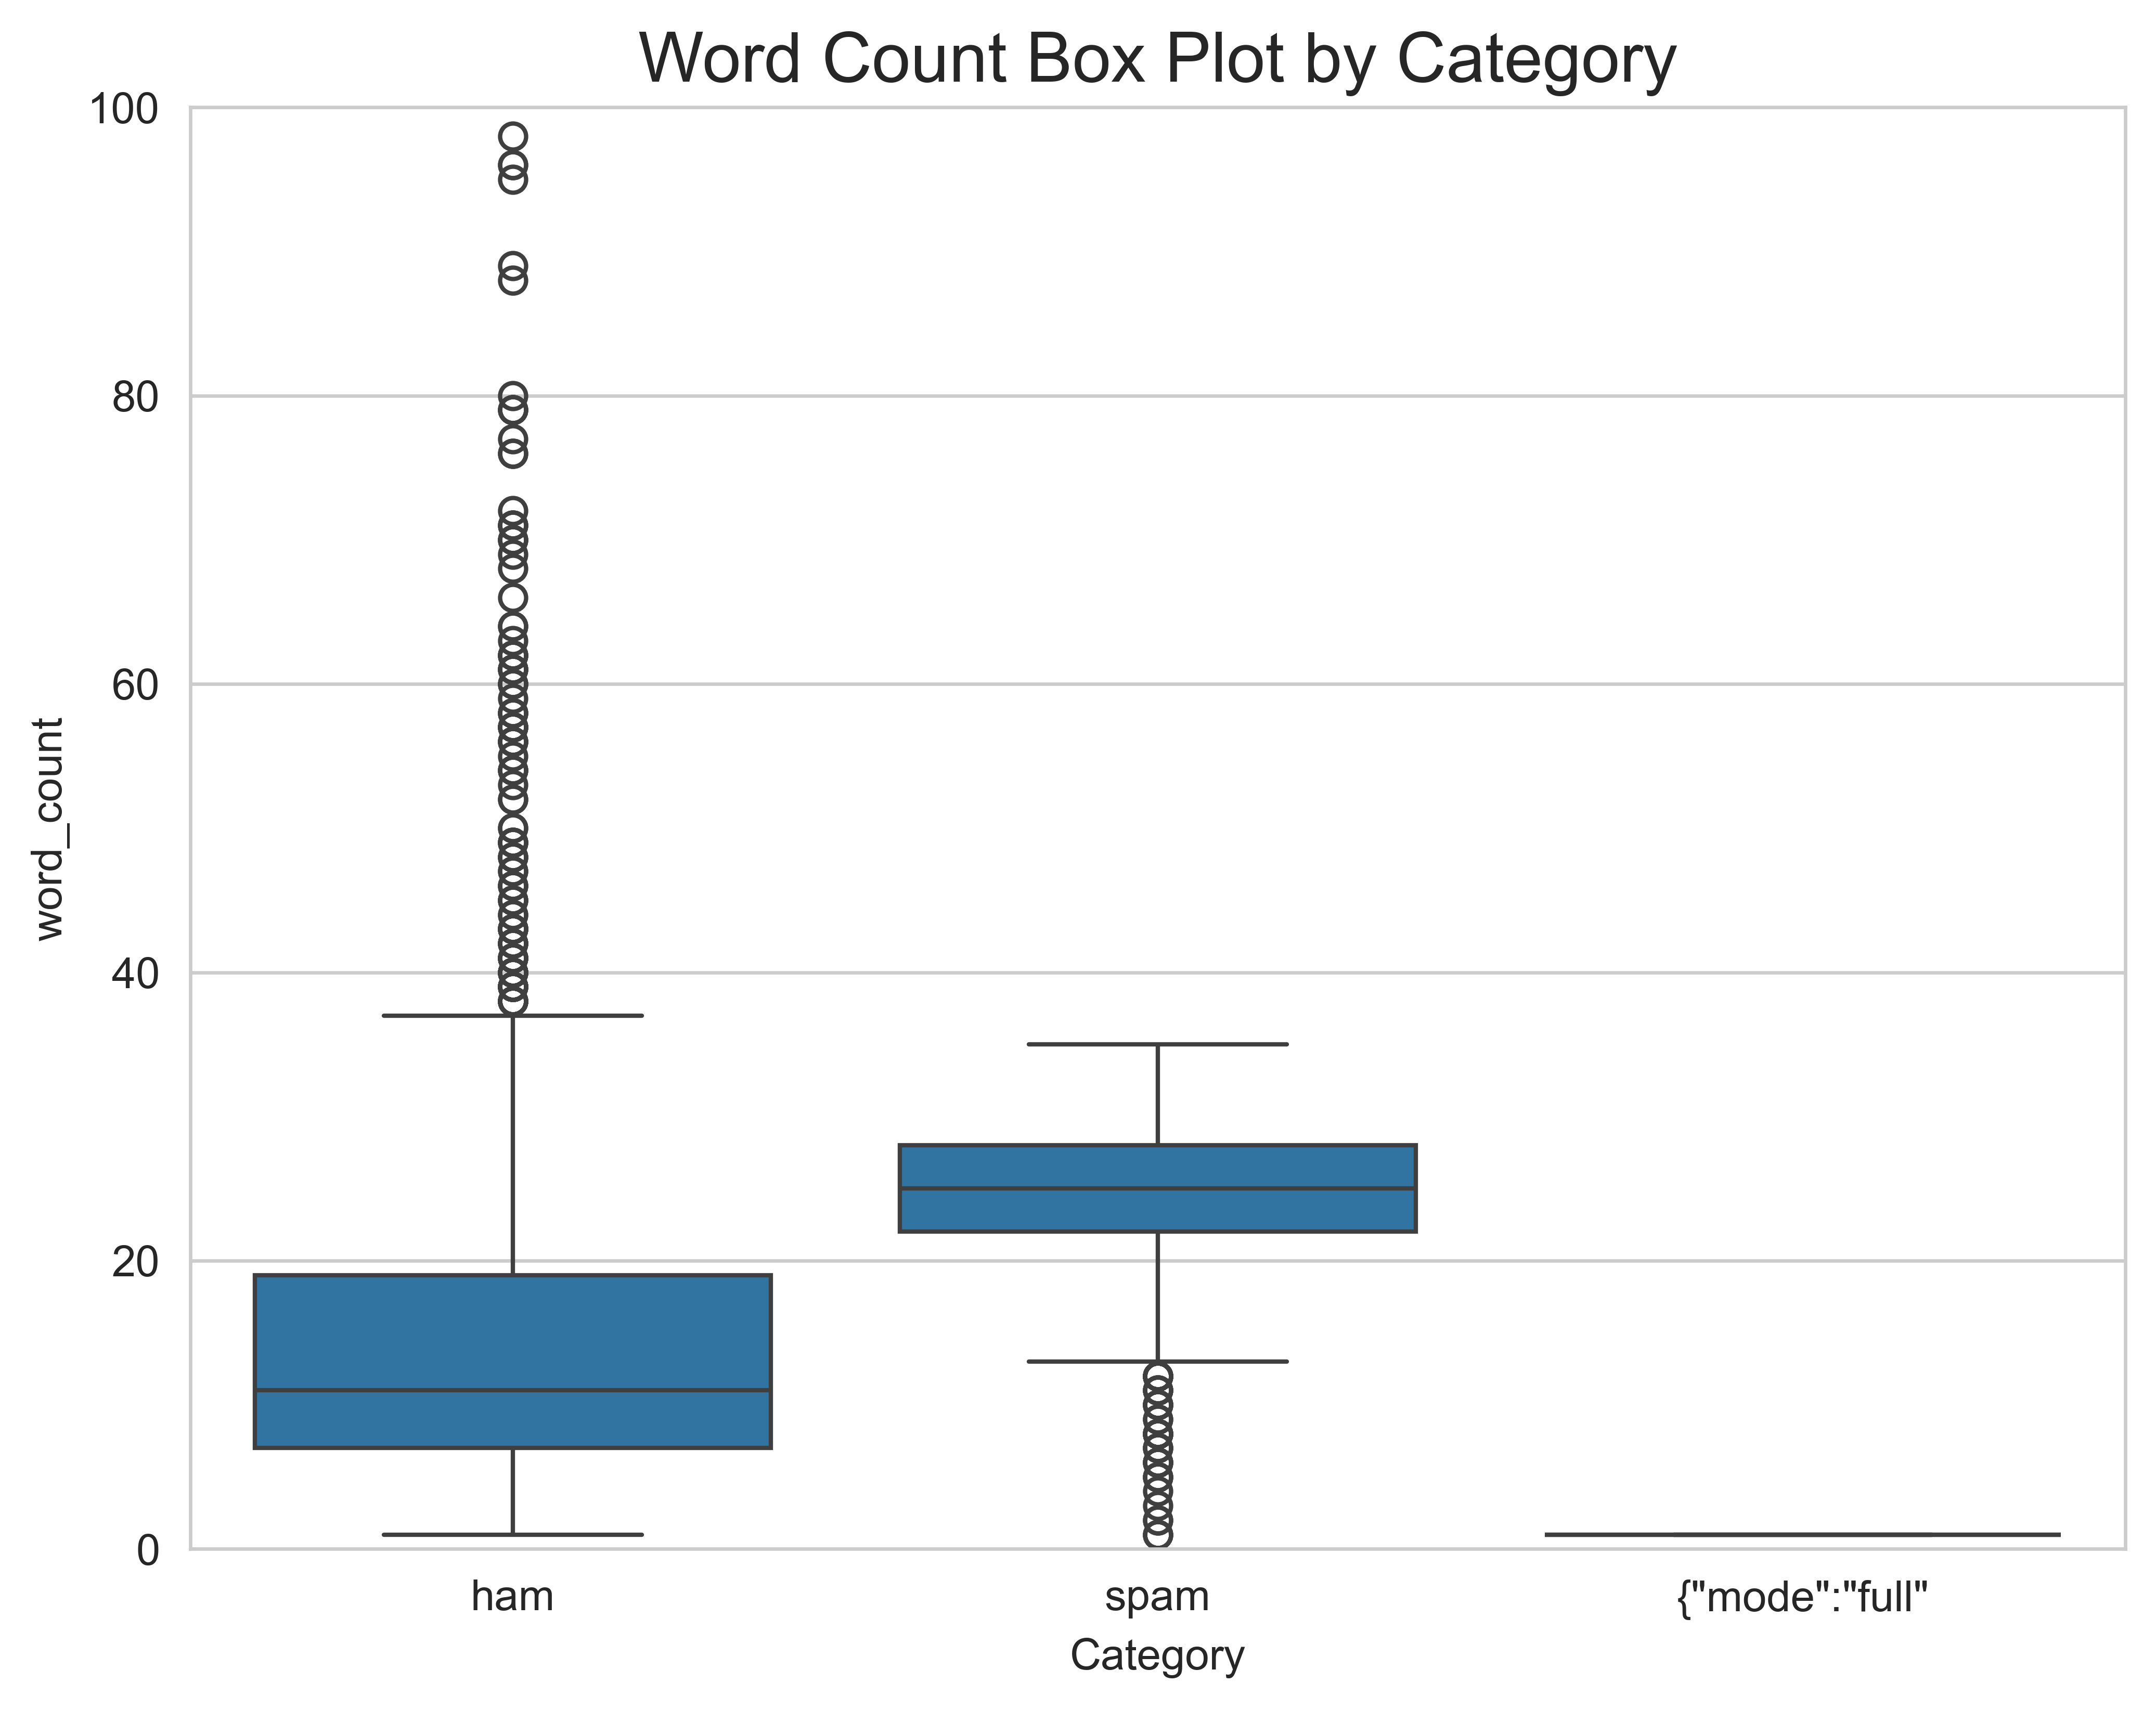
\includegraphics[width=0.7\textwidth]{png/spam_boxplot.png}
\caption{Word Count Box Plot - Email Spam}
\end{figure}

\begin{figure}[H]
\centering
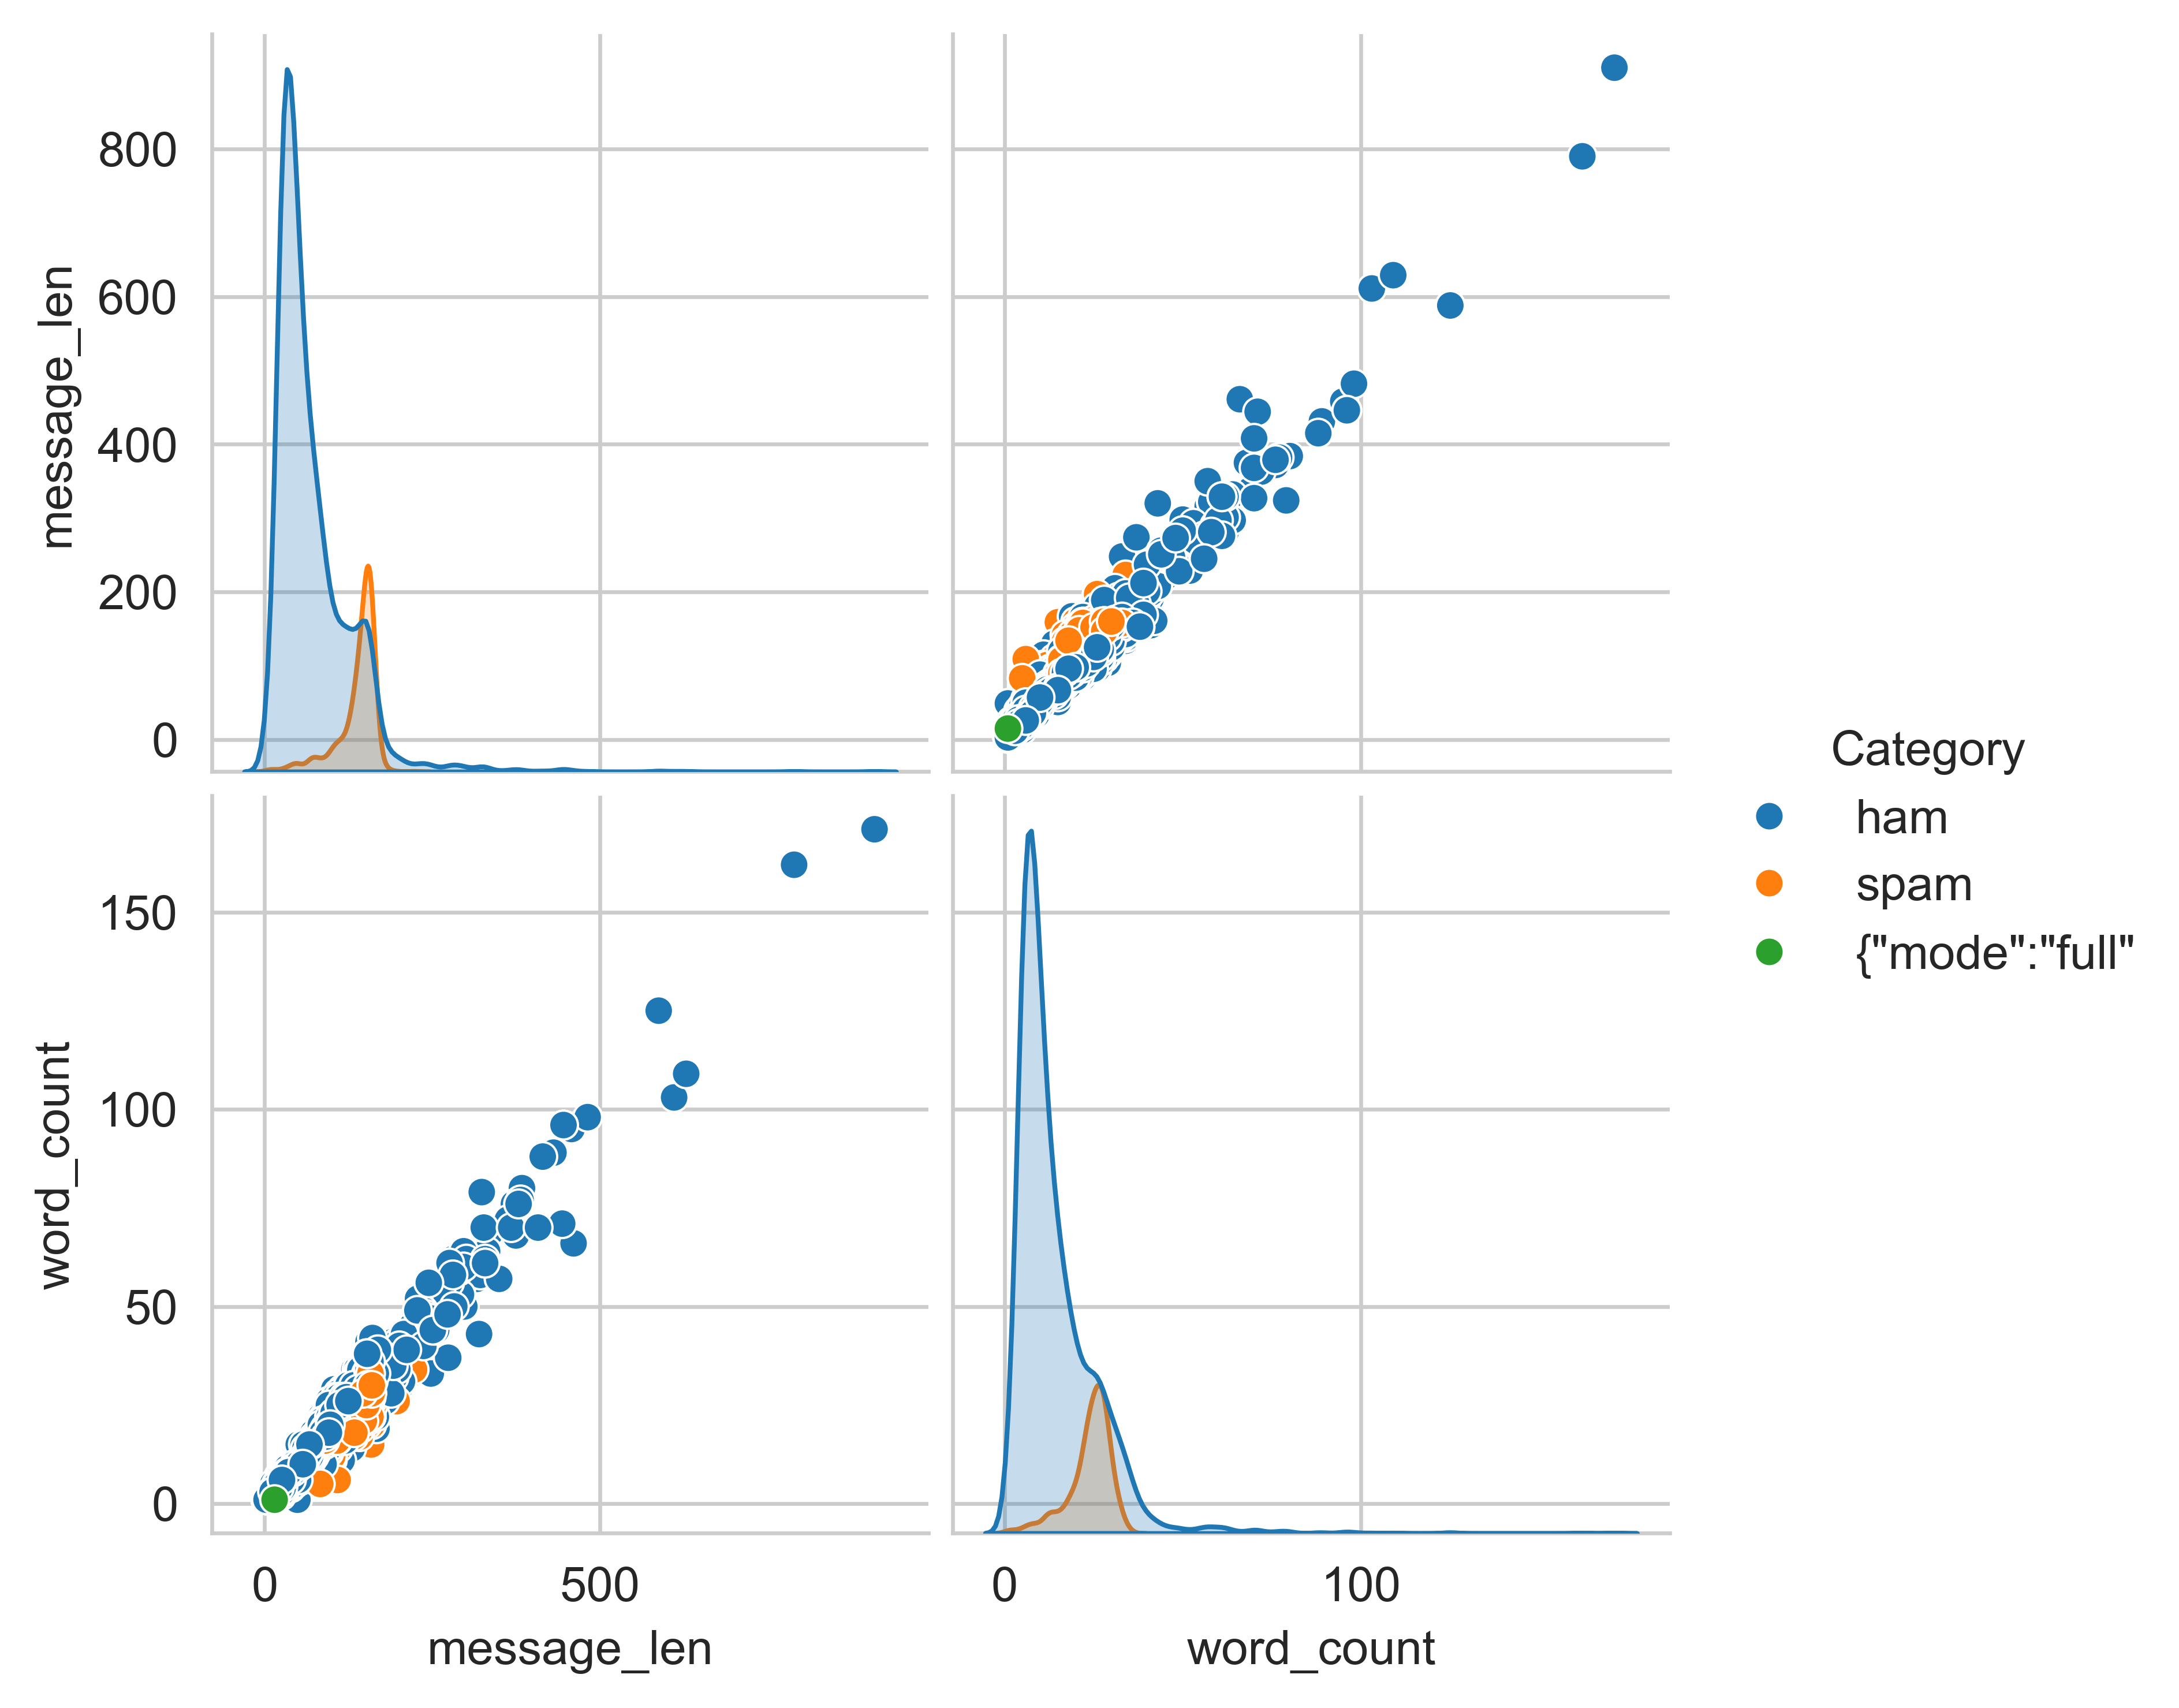
\includegraphics[width=0.85\textwidth]{png/spam_pairplot.png}
\caption{Pair Plot Analysis - Email Spam}
\end{figure}

\subsection*{3.5 Handwritten Character Recognition / MNIST}

\begin{figure}[H]
\centering
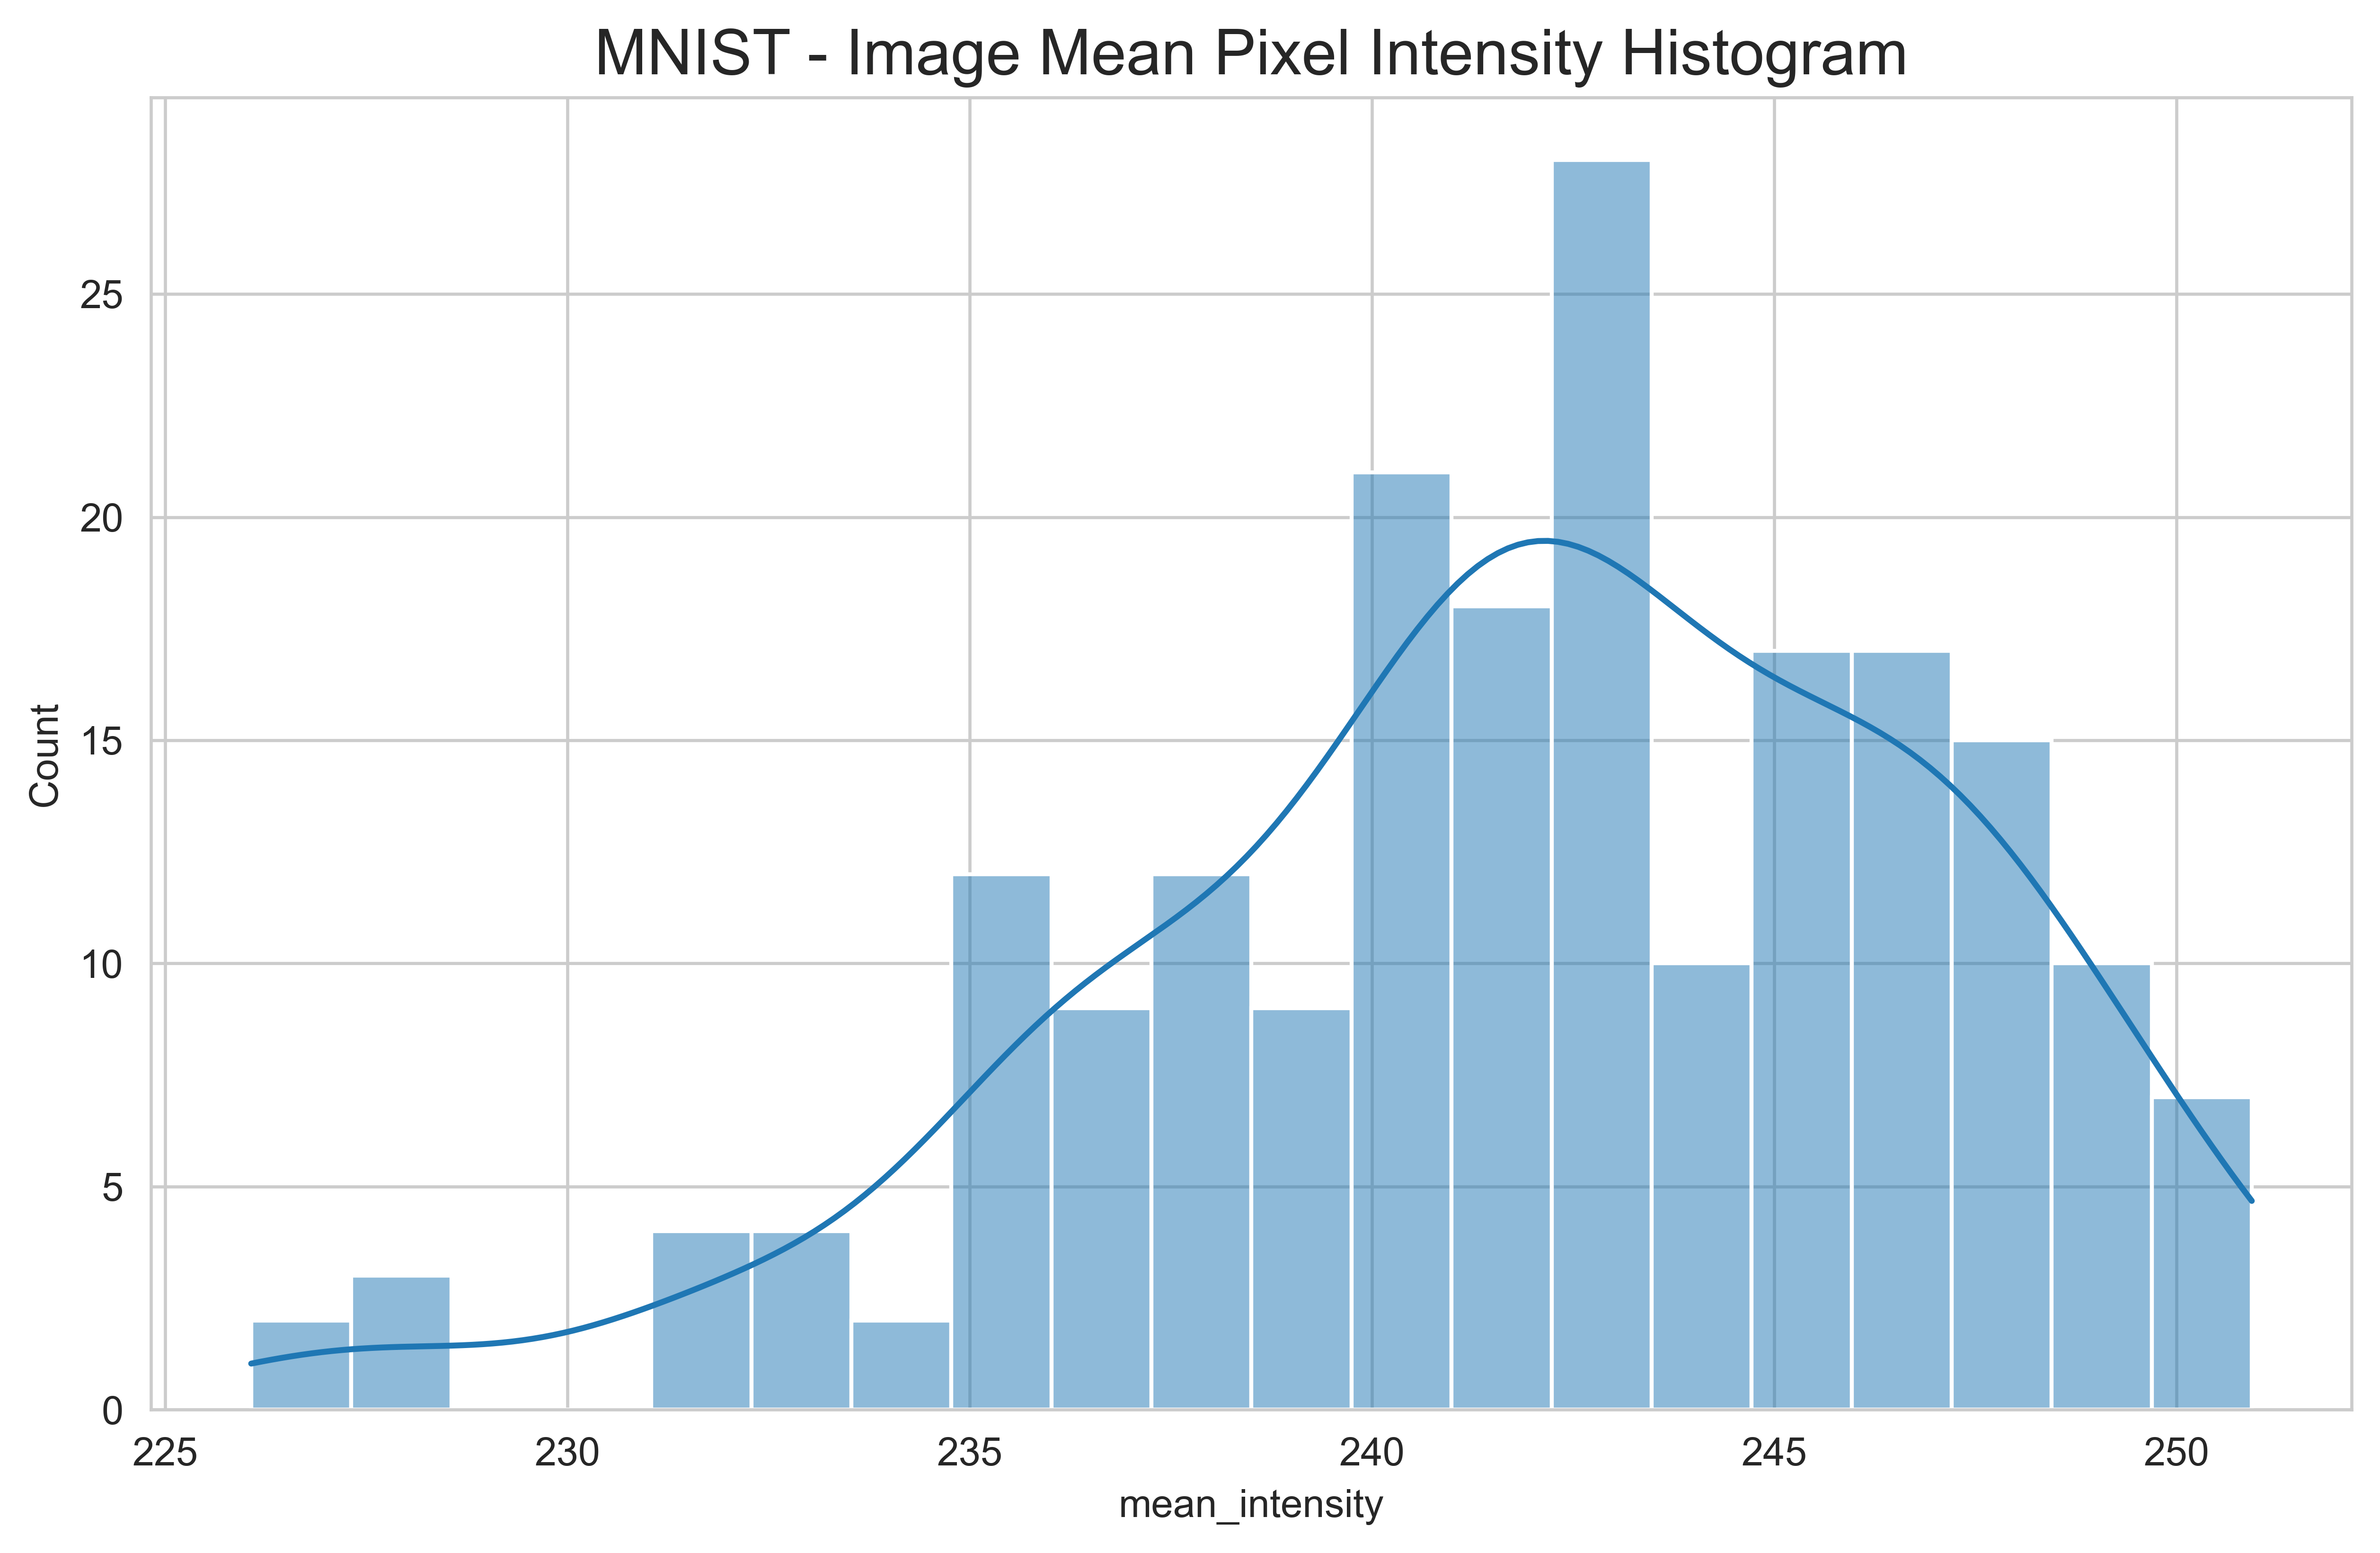
\includegraphics[width=0.8\textwidth]{png/mnist_hist_intensity.png}
\caption{Pixel Intensity Histogram - MNIST}
\end{figure}

\begin{figure}[H]
\centering
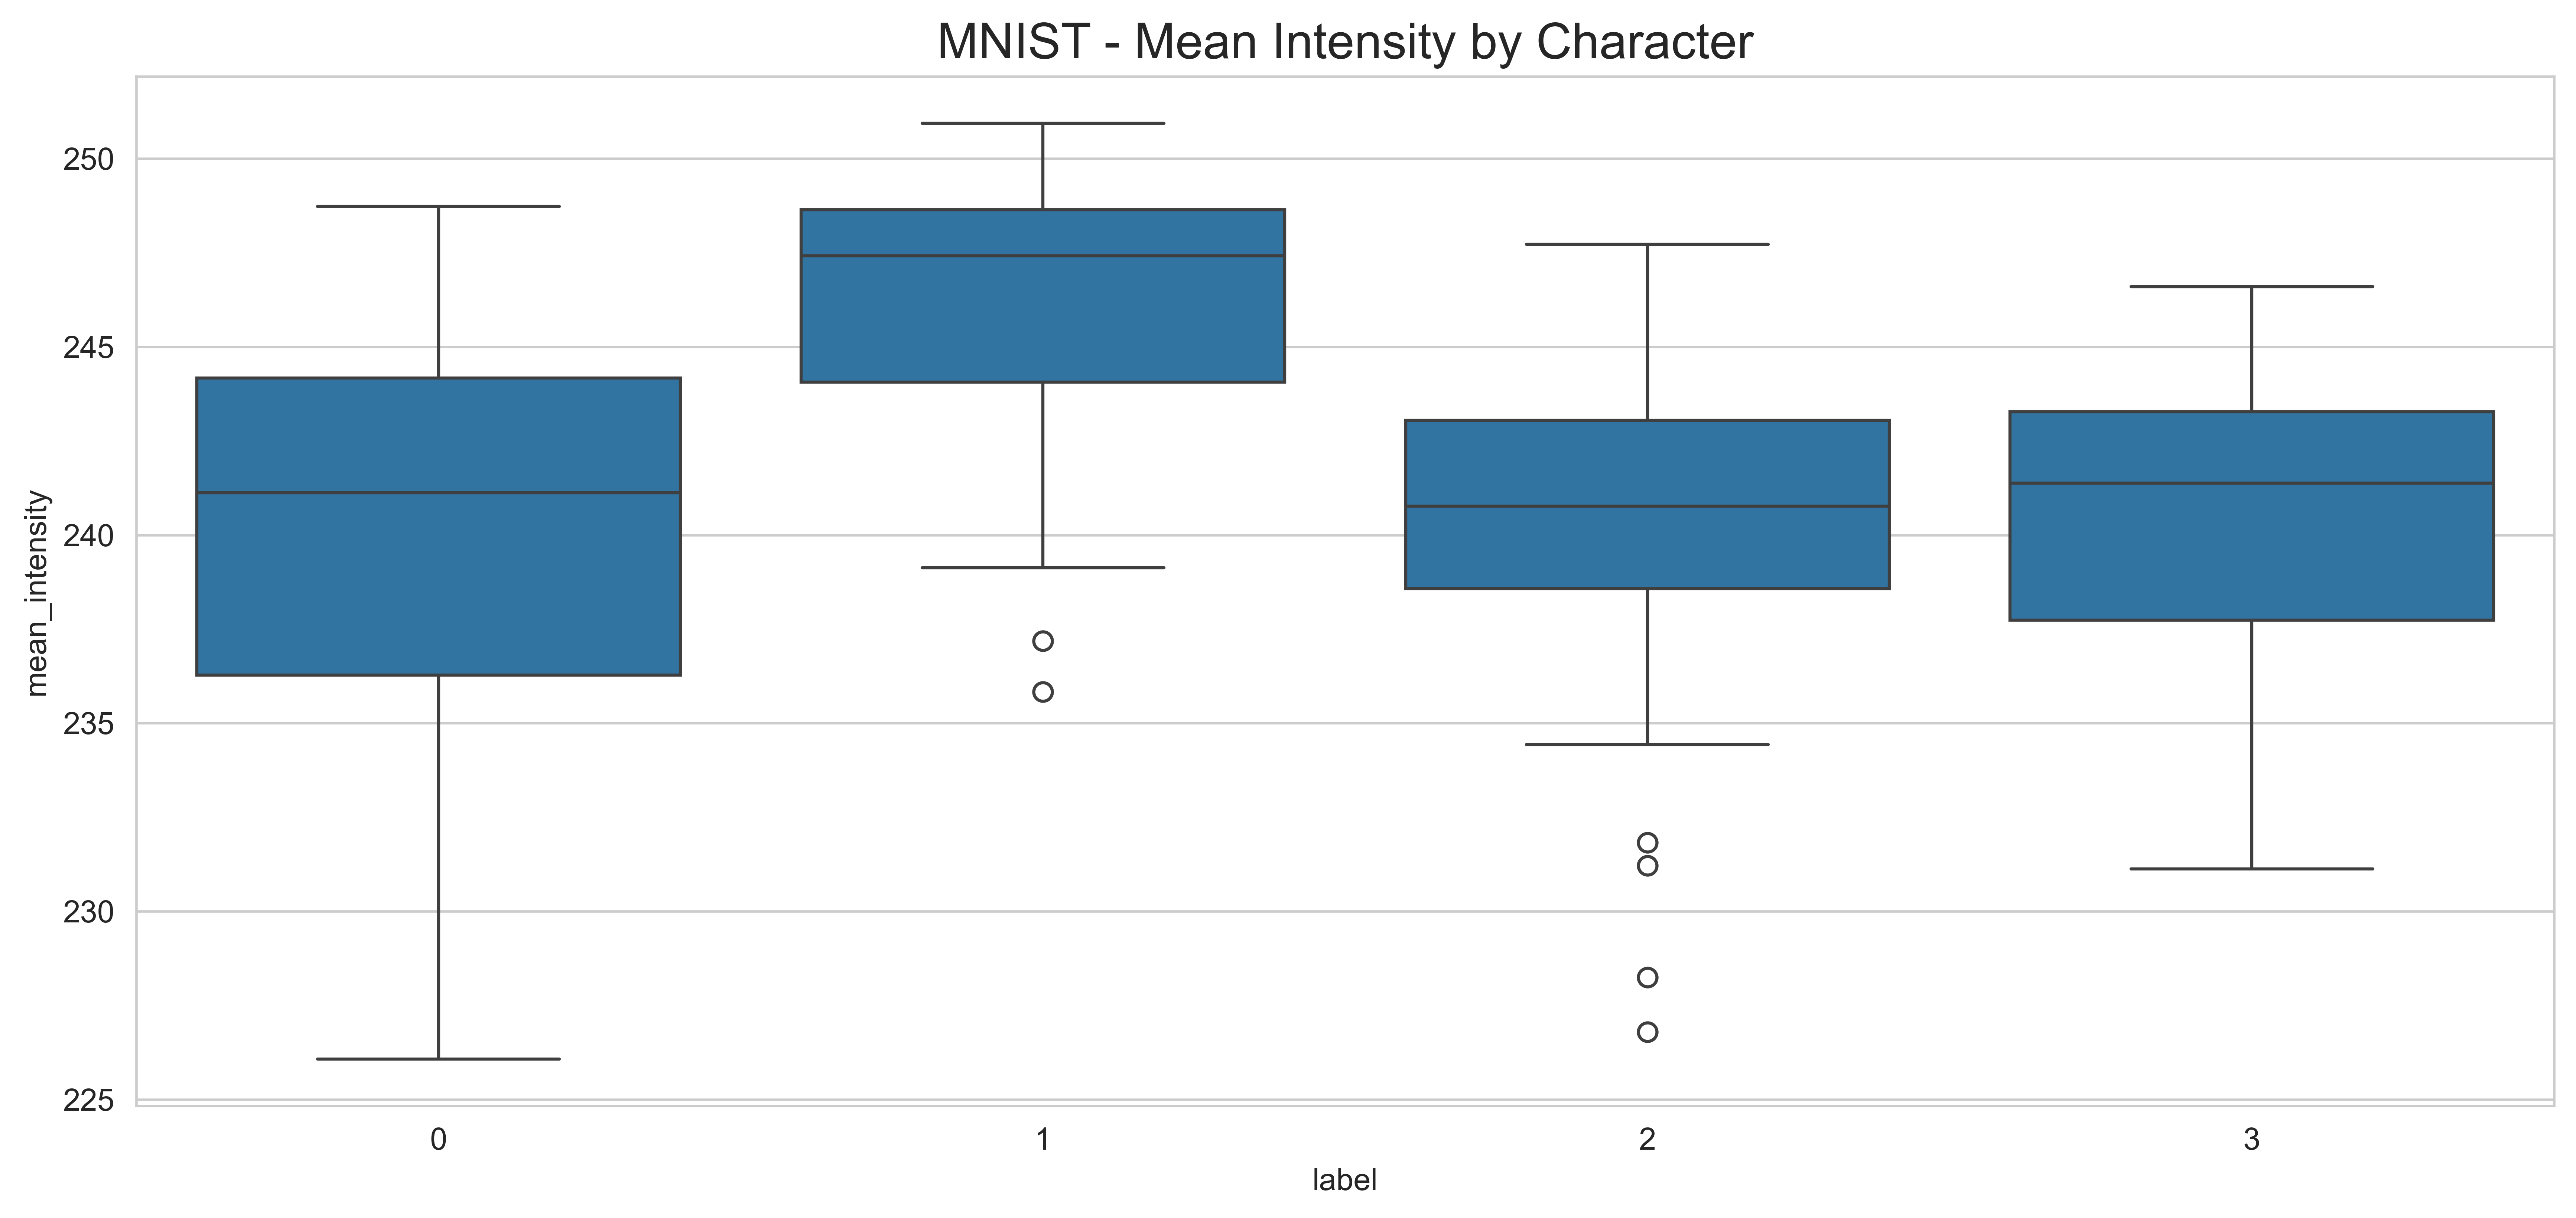
\includegraphics[width=0.8\textwidth]{png/mnist_boxplot.png}
\caption{Mean Intensity Box Plot - MNIST}
\end{figure}

\begin{figure}[H]
\centering
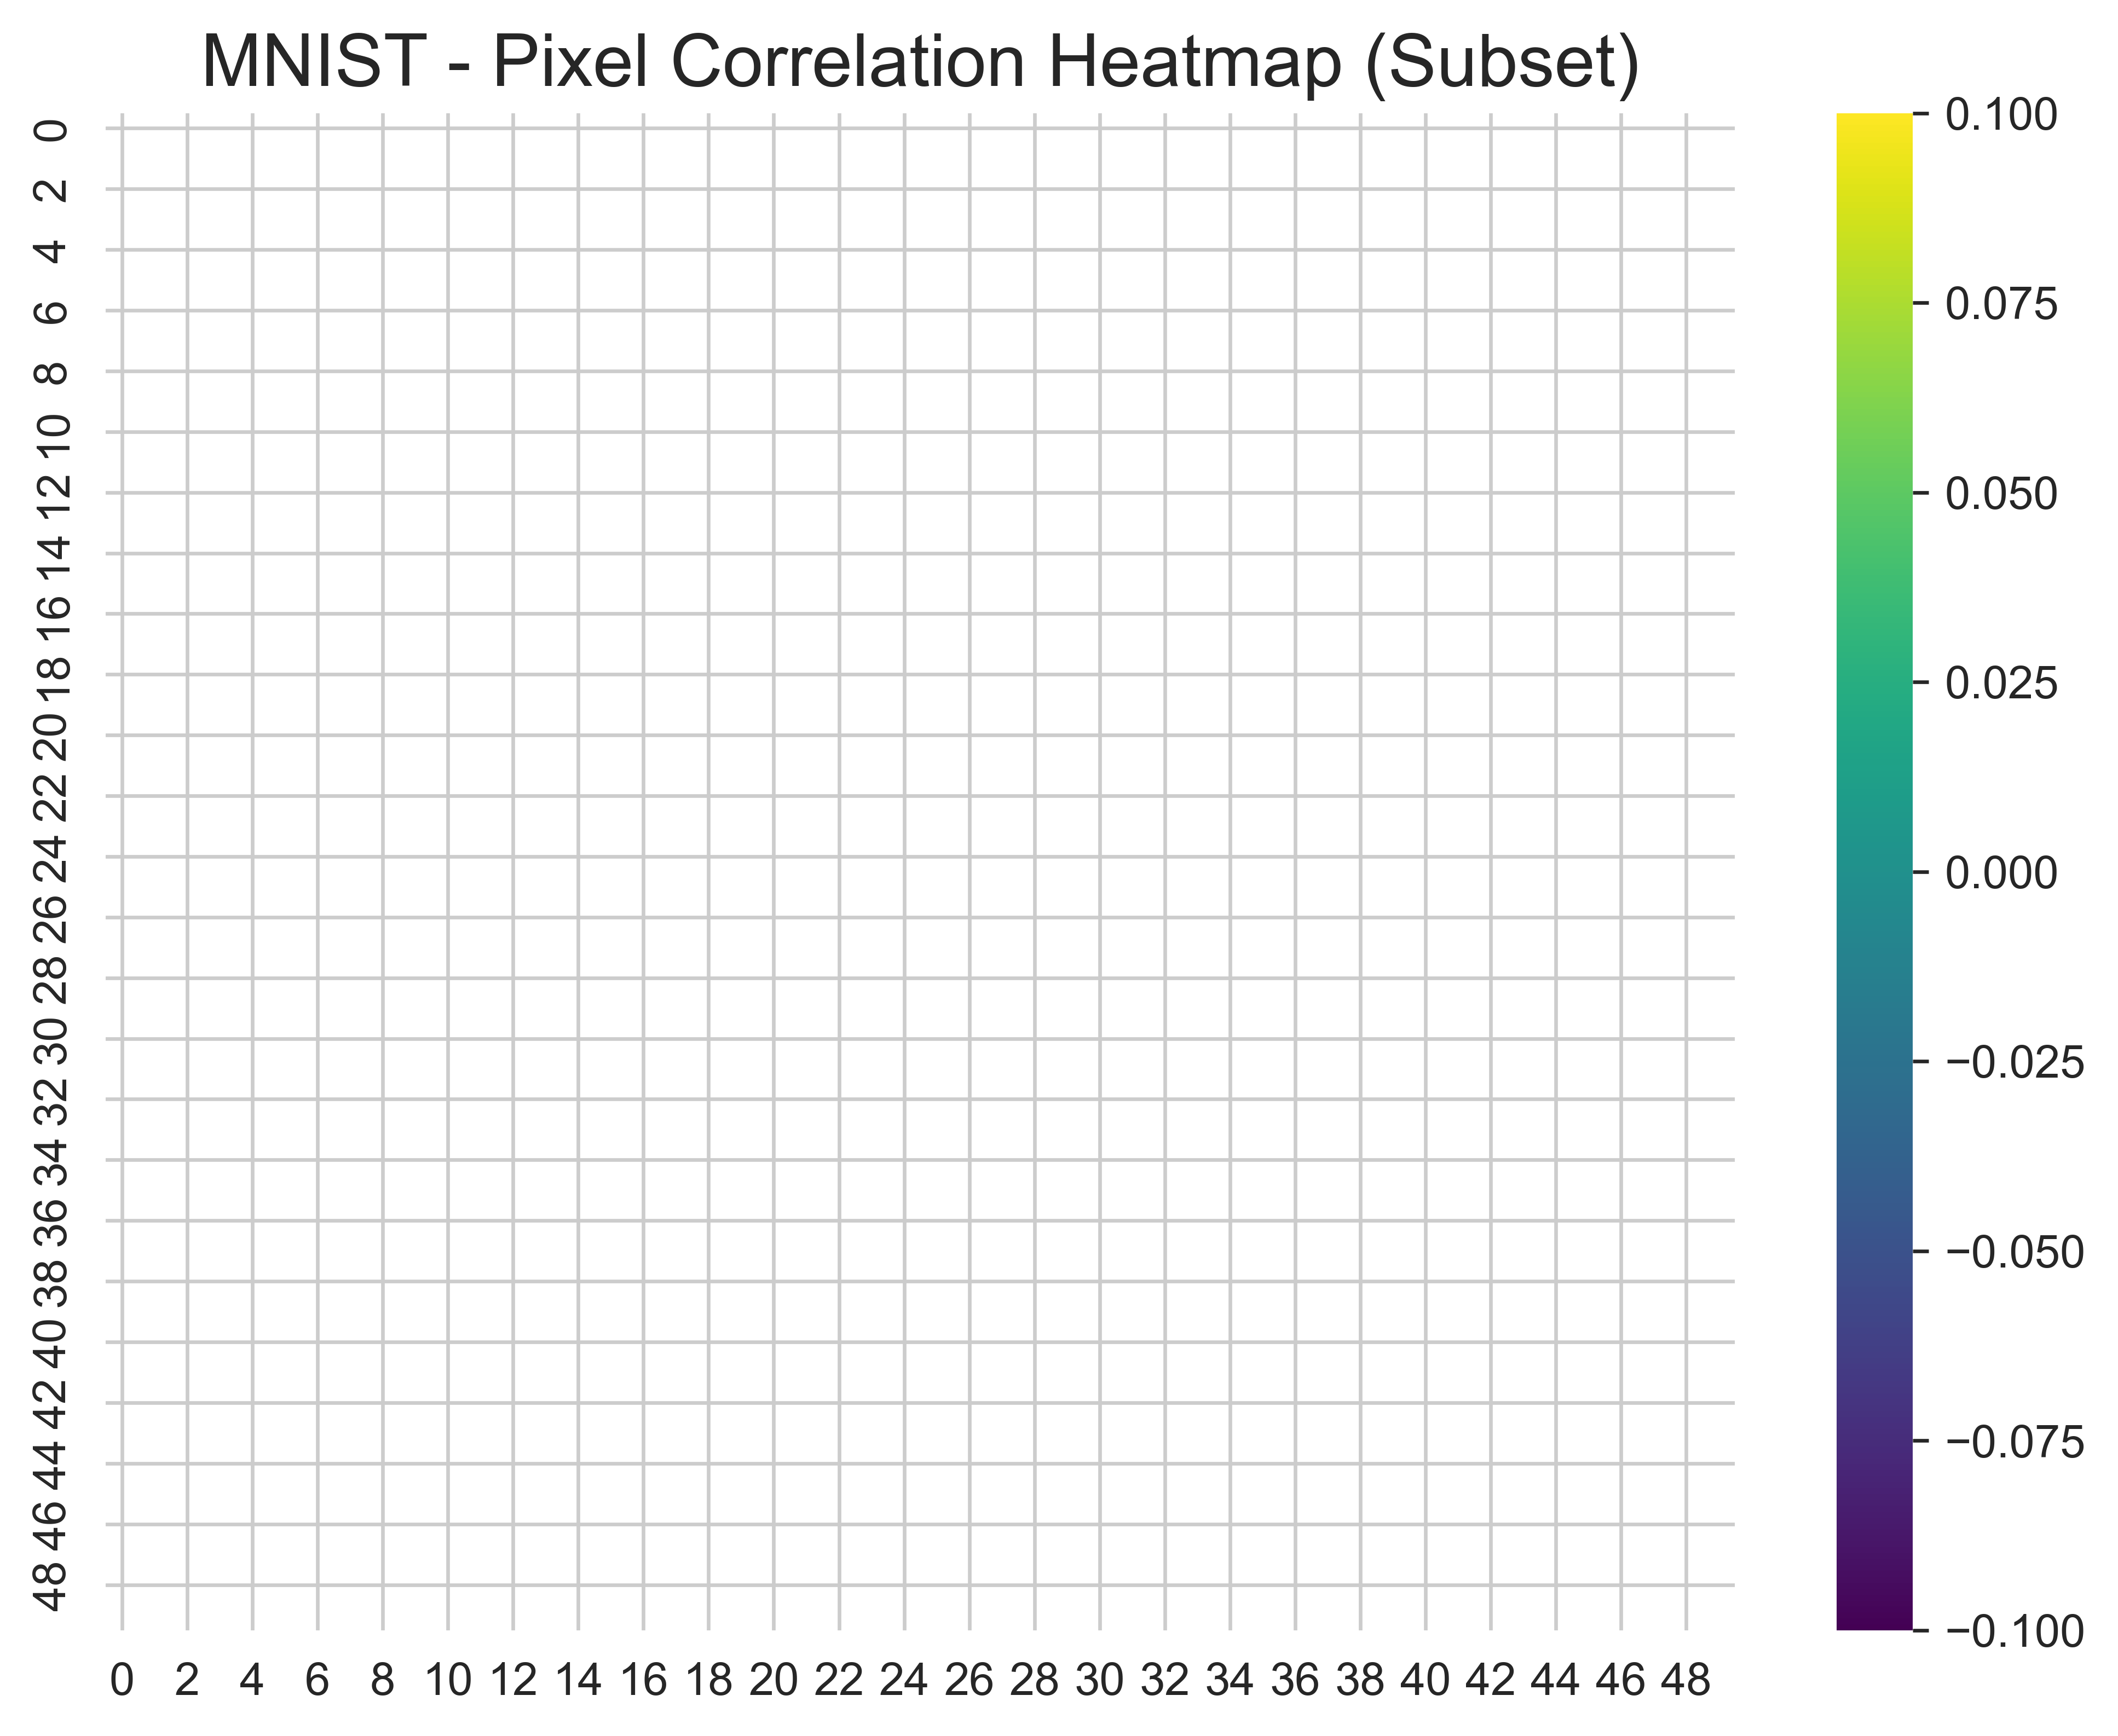
\includegraphics[width=0.7\textwidth]{png/mnist_heatmap.png}
\caption{Pixel Correlation Heatmap (Subset) - MNIST}
\end{figure}

\begin{figure}[H]
\centering
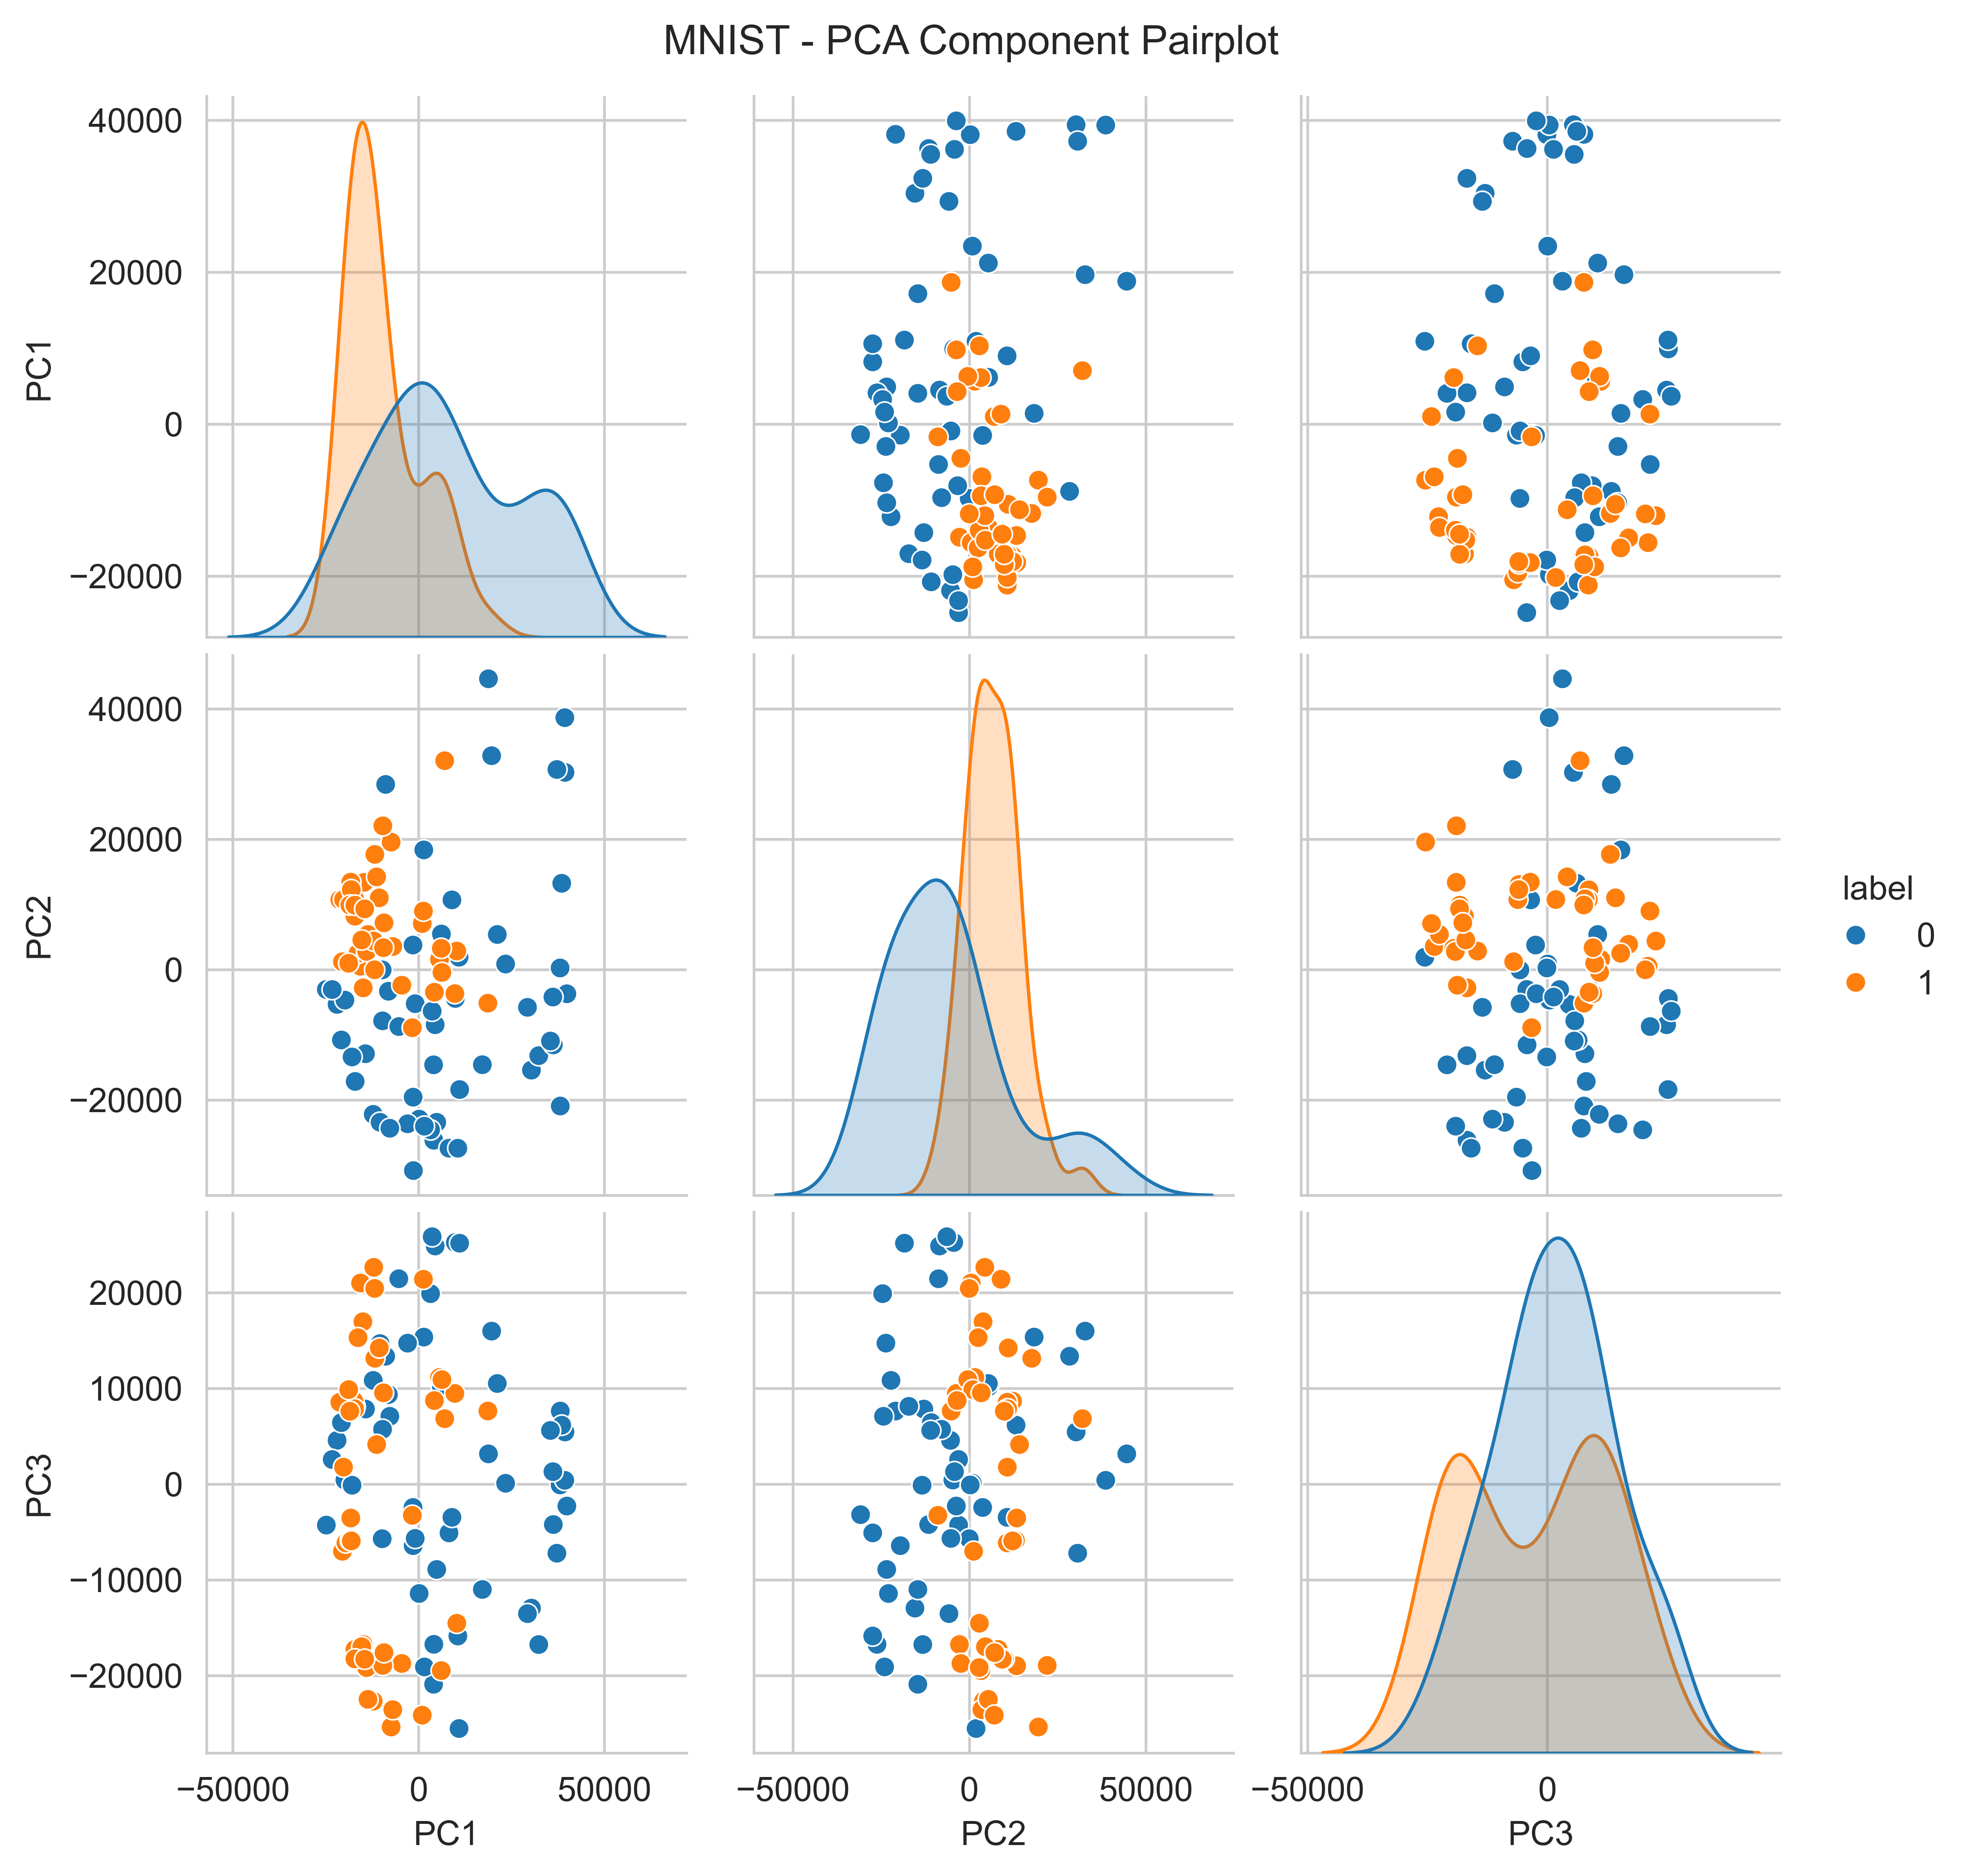
\includegraphics[width=0.85\textwidth]{png/mnist_pca_pairplot.png}
\caption{PCA Components Pair Plot - MNIST}
\end{figure}

% --------------------------------------------------

\section*{4. ML Task Analysis}

\begin{table}[H]
\centering
\caption{Machine Learning Task Analysis for Each Dataset}
\begin{tabular}{|p{4cm}|p{3cm}|p{3.5cm}|p{3.5cm}|}
\hline
\textbf{Dataset} & \textbf{Type of ML Task} & \textbf{Feature Selection Technique} & \textbf{Suitable ML Algorithm} \\ \hline
Iris Dataset & Multi-class Classification & Correlation Analysis, PCA, Variance Analysis & Logistic Regression, Decision Tree, K-Nearest Neighbors, Support Vector Machine \\ \hline
Loan Amount Prediction & Regression & Correlation Matrix, Feature Importance, Variance Inflation Factor & Linear Regression, Ridge Regression, Random Forest Regressor, Gradient Boosting \\ \hline
Predicting Diabetes & Binary Classification & Chi-square Test, Mutual Information, Recursive Feature Elimination & Logistic Regression, Random Forest, Support Vector Machine, Naive Bayes \\ \hline
Classification of Email Spam & Binary Classification & TF-IDF Vectorization, Chi-square Test, Information Gain & Naive Bayes, Support Vector Machine, Logistic Regression, Random Forest \\ \hline
Handwritten Character Recognition / MNIST & Multi-class Classification & Principal Component Analysis, Variance Threshold, Feature Extraction & Convolutional Neural Network, Random Forest, Support Vector Machine, K-Nearest Neighbors \\ \hline
\end{tabular}
\end{table}

% --------------------------------------------------

\section*{5. Key Observations}

\subsection*{5.1 Data Loading and Preprocessing}
\begin{itemize}
\item Successfully loaded all datasets using appropriate Python libraries including Pandas for structured data and sklearn.datasets for benchmark datasets
\item Systematically identified and quantified missing values across all datasets and implemented appropriate imputation strategies
\item Performed necessary data type conversions to ensure compatibility with machine learning algorithms
\item Applied standardization and normalization techniques to numerical features to ensure uniform scale and improve model convergence
\item Handled categorical variables through appropriate encoding techniques where applicable
\end{itemize}

\subsection*{5.2 Exploratory Data Analysis}
\begin{itemize}
\item Conducted comprehensive analysis of class distributions to identify potential imbalances that may require sampling techniques
\item Examined inter-feature correlations using correlation matrices and identified multicollinearity issues
\item Detected outliers using multiple statistical methods including box plots, Z-scores, and interquartile range analysis
\item Visualized feature distributions through histograms, kernel density plots, and quantile-quantile plots to assess normality
\item Investigated relationships between features and target variables using scatter plots and pair plots
\item Analyzed feature importance and contribution to model predictions
\end{itemize}

\subsection*{5.3 ML Task Identification}
\begin{itemize}
\item Accurately distinguished between classification and regression tasks based on target variable characteristics and problem statements
\item Differentiated between binary and multi-class classification problems and their respective evaluation metrics
\item Recommended appropriate machine learning algorithms considering dataset size, dimensionality, and computational constraints
\item Identified suitable feature selection and dimensionality reduction techniques aligned with specific task requirements
\item Considered algorithm interpretability requirements for different application domains
\item Evaluated trade-offs between model complexity and performance for each dataset
\end{itemize}

% --------------------------------------------------

\section*{6. Conclusion}
This comprehensive experiment provided extensive hands-on experience with essential Python libraries that form the foundation of modern machine learning workflows. Through systematic loading, preprocessing, exploration, and visualization of five diverse datasets spanning various domains, valuable insights were gained into different machine learning task types and their corresponding algorithmic approaches. The exploratory data analysis revealed critical patterns, correlations, and statistical characteristics that directly inform algorithm selection, hyperparameter tuning, and preprocessing strategies. The experiment successfully demonstrated the importance of understanding data characteristics before model development and highlighted the interconnected nature of data preprocessing, feature engineering, and algorithm selection in building effective machine learning solutions.

\section*{References}
\begin{itemize}
\item Numpy – Official Documentation: https://numpy.org/doc/
\item Pandas – Official Documentation: https://pandas.pydata.org/docs/
\item Scikit-learn – Official Documentation: https://scikit-learn.org/stable/
\item Matplotlib – Official Documentation: https://matplotlib.org/stable/contents.html
\item Scipy – Official Documentation: https://docs.scipy.org/doc/
\item UCI Machine Learning Repository: https://archive.ics.uci.edu/ml/
\item Kaggle Datasets: https://www.kaggle.com/datasets
\end{itemize}

\end{document}